%%%%%%%%%%%%%%%%%%%%%%%%%%%%%%%%%%%%%%%%%%%%%%%%%%%%%%%%%%%%%%%%%%%%%%%%%%%%%%%
% Uni Duesseldorf
% Lehrstuhl fuer Datenbanken and Informationssysteme
% Vorlage fuer Bachelor-/Masterarbeiten
% Optimiert fuer den Original-Latex-Kompiler LATEX.EXE (LaTeX=>PS=>PDF)
% Version 1.4 - 2.3.2010
%%%%%%%%%%%%%%%%%%%%%%%%%%%%%%%%%%%%%%%%%%%%%%%%%%%%%%%%%%%%%%%%%%%%%%%%%%%%%%%

%%%%%%%%%%%%%%%%%%%%%%%%%%%%%%%%%%%%%%%%%%%%%%%%%%%%%%%%%%%%%%%%%%%%%%%%%%%%%%%
%%%%%%%%%%% BEGINN EINSTELLUNG FUER DIE ARBEIT. UNBEDINGT ERFORDERLICH! %%%%%%%
%%%%%%%%%%%%%%%%%%%%%%%%%%%%%%%%%%%%%%%%%%%%%%%%%%%%%%%%%%%%%%%%%%%%%%%%%%%%%%%
% Geben Sie Ihren Namen hier an
\newcommand{\bearbeiter}{Alina Elterman}

% Geben Sie hier den Titel Ihrer Arbeit an
\newcommand{\titel}{Metrische Dimension Spezieller Graphklassen}

% Geben Sie das Datum des Beginns and Ende der Bachelorarbeit ein
\newcommand{\beginndatum}{28. Juni 2012}
\newcommand{\abgabedatum}{?. Dezember 2012}

% Geben Sie die Namen des Erst- and Zweitgutachters an
\newcommand{\erstgutachter}{Prof. Dr. Egon Wanke}
\newcommand{\zweitgutachter}{PD Dr. Frank Gurski}

% Falls Sie die Arbeit zweiseitig ausdrucken wollen,
% benutzen Sie die folgende Zeile mit
% \AN fuer zweiseitigen Druck
% \AUS fuer einseitigen Druck
\newcommand{\zweiseitig}{\AUS}

% Falls die Arbeit in englischer Sprache verfasst 
% werden soll, dann benutzen Sie die folgende Zeile mit
% englisch fuer englische Sprache
% deutsch fuer deutsche Sprache
\newcommand{\sprache}{deutsch}
%%%%%%%%%%%%%%%%%%%%%%%%%%%%%%%%%%%%%%%%%%%%%%%%%%%%%%%%%%%%%%%%%%%%%%%%%%%%%%%%%
%%%%%%%%%%%%%%%%%%%%%%%%%%%%%%% ENDE EINSTELLUNGEN %%%%%%%%%%%%%%%%%%%%%%%%%%%%%%
%%%%%%%%%%%%%%%%%%%%%%%%%%%%%%%%%%%%%%%%%%%%%%%%%%%%%%%%%%%%%%%%%%%%%%%%%%%%%%%%%

% Die folgende Zeile NICHT EDITIEREN oder loeschen
% (Zum Ab�ndern der BA-Vorlage in eine MA-Vorlage muessen sie
% jedoch die Datei titelmakros1.tex selbst editieren.)
%%%%%%%%%%%%%%%%%%%%%%%%%%%%%%%%%%%%%%%%%%%%%%%%%%%%%%%%%%%
% Obere Titelmakros. Editieren Sie diese Datei nur, wenn
% Sie sich ABSOLUT sicher sind, was Sie da tun!!!
% (Z.B. zum Abaendern der BA-Vorlage in eine MA-Vorlage)
% Uni Duesseldorf
% Lehrstuhl fuer Datenbanken und Informationssysteme
% Version 2.2 - 2.3.2010
%%%%%%%%%%%%%%%%%%%%%%%%%%%%%%%%%%%%%%%%%%%%%%%%%%%%%%%%%%%
\newcommand{\AN}{twoside}
\newcommand{\AUS}{}
%\newcommand{\englisch}{}
%\newcommand{\deutsch}{\usepackage[german]{babel}}

%% Die folgenden auskommentierten Optionen dienen der automatischen
%% Erkennung des Latex-Kompilers und dem Setzen der davon abh�ngigen
%% Einstellungen. Bei Problem z.B. mit dem Einbinden von verschiedenen
%% Grafiktypen bei Verwendung von PdfLatex oder Latex, einfach die
%% verschiedenen \usepackage(s) ausprobieren. (Mit diesen Einstellungen
%% funktionierte diese Vorlage bei der Verwenundg von latex.exe als
%% Kompiler bei den meisten Studierenden.)

%\newif\ifpdf \ifx\pdfoutput\undefined
%\pdffalse % we are not running pdflatex
%\else
%\pdfoutput=1 % we are running pdflatex
%\pdfcompresslevel=9 % compression level for text and image;
%\pdftrue \fi[cleardoublepage=plain]

\documentclass[11pt,a4paper,pointlessnumbers, \zweiseitig]{scrreprt}



%\usepackage[iso]{umlaute}
%\usepackage[latin1]{inputenc}
\usepackage{palatino} % palatino Schriftart
%\usepackage{makeidx} % um ein Index zu erstellen
\usepackage{tocbibind}
\usepackage[T1]{fontenc} %fuer richtige Trennung bei Umlauten
\usepackage{fancybox} % fuer die Rahmen
\usepackage{shortvrb}
\usepackage{ifthen}
%\ifthenelse{\equal{\sprache}{deutsch}}{\usepackage[ngerman]{babel}}{}
\usepackage[utf8]{inputenc}
\usepackage[ngerman]{babel}
\usepackage{lmodern} 
\usepackage{amsmath}
\usepackage{oldgerm}
\usepackage{amssymb}
\usepackage{pdfpages}
\usepackage{hyperref}
%\usepackage{fancyheadings}
\usepackage{fancyhdr}
\usepackage{amsfonts}
%\usepackage{complexity}
\usepackage{amsthm}
\usepackage{color}
\usepackage{caption}
%\usepackage{stmaryrd}
\usepackage{graphicx}
\usepackage{graphics}
\usepackage{nomencl}
\usepackage[normalem]{ulem} 
\usepackage{verbatim}
\usepackage{ulsy}
\usepackage{floatflt}
\usepackage{float}
\usepackage{tikz}
\usepackage{pgf}
\usepackage{bbding}
\usepackage{nicefrac}
\usepackage{stmaryrd}
\usepackage{tabularx}
\usepackage{multirow}
\usepackage{array}
\usepackage{algorithm}
\usepackage{algorithmic}
% \usepackage[disable]{todonotes}				% alle todo-Anmerkungen ausblenden
\usepackage[german, color=yellow!40, colorinlistoftodos, textsize=footnotesize, shadow]{todonotes}
\usetikzlibrary{arrows,automata,petri,shapes,snakes}


\newcommand{\markup}[1]{\uline{#1}}
% Befehl umbenennen in abk
\let\abk\nomenclature

\usepackage{a4wide} % ganze A4 Weite verwenden

%\ifpdf
%\usepackage[pdftex,xdvi]{graphicx}
%\usepackage{thumbpdf} %thumbs fuer Pdf
%\usepackage[pdfstartview=FitV]{hyperref} %anklickbares Inhaltsverzeichnis
%\else
%\usepackage[dvips,xdvi]{graphicx}
%\usepackage{hyperref} %anklickbares Inhaltsverzeichnis
%\fi

%%%%%%%%%%%%%%%%%%%%%%% Massangaben fuer die Arbeit %%%%%%%%%%%%%%%
\setlength{\textwidth}{15cm}

\setlength{\oddsidemargin}{35mm}
\setlength{\evensidemargin}{25mm}

\addtolength{\oddsidemargin}{-1in}
\addtolength{\evensidemargin}{-1in}

%\makeindex
% Umgebungen f"ur S�tze usw.
\clearpage{\pagestyle{empty}\cleardoublepage}
\newtheorem{bem}{Bemerkung}
\newtheorem{definition}{Definition}
\newtheorem{bezeichnungen}{Bezeichnungen}
\newtheorem{fakt}{Fakt}
\newtheorem{beispiel}{Beispiel}
\newtheorem{bsp}{Beispiel}
\newtheorem{satz}{Satz}
\newtheorem{lem}{Lemma}
\newtheorem{folg}{Folgerung}
\newtheorem{idee}{Idee}
\newtheorem{corollary}{Korollar}
\floatname{algorithm}{Algorithmus}
\renewcommand{\algorithmicrequire}{\textbf{Eingabe:}}
\renewcommand{\algorithmicensure}{\textbf{Ausgabe:}}
\newenvironment{defi}[1][]{\ifthenelse{\equal{#1}{}}{\definition}{\definition[#1]}\rm}{\enddefinition}
\newcommand{\EP}[3]{
\medskip
\begin{center}
\begin{tabularx}{0.92\textwidth}{ll}
\hline\hline
\multicolumn{2}{c}{\textsc{#1}} \\
\hline
\em{Gegeben:}& #2\\
\em{Frage:}& #3 \\
\hline\hline
\end{tabularx}
\end{center}
\medskip}

\newcommand{\MP}[3]{
\medskip
\begin{center}
\begin{tabularx}{0.92\textwidth}{ll}
\hline\hline
\multicolumn{2}{c}{\textsc{#1}} \\
\hline
\em{Gegeben:}& #2\\
\em{Gesucht:}& #3 \\
\hline\hline
\end{tabularx}
\end{center}
\medskip}

%definition of new commands
\newcommand{\vsp}{\vspace{3mm}}
\newcommand{\impl}[1]{\overset{\text{#1}}{\implies}}
\newcommand{\notimplleft}[1]{\overset{\text{#1}}{\not\Leftarrow}}
\renewcommand{\figurename}{Abbildung}
\renewcommand{\tablename}{Tabelle}
\renewcommand{\contentsname}{Inhaltsverzeichnis}
\renewcommand{\listfigurename}{Abbildungsverzeichnis}
\renewcommand{\listtablename}{Tabellenverzeichnis}
\renewcommand\bibname{Literaturverzeichnis}
\begin{document}

%\setcounter{secnumdepth}{4} %Nummerieren bis in die 4. Ebene
%\setcounter{tocdepth}{4} %Inhaltsverzeichnis bis zur 4. Ebene

\pagestyle{headings}
\thispagestyle{empty}
\sloppy % LaTeX ist dann nicht so streng mit der Silbentrennung
%\MakeShortVerb{\�}

\parindent0mm
\parskip0.5em


{
\textwidth170mm 
\oddsidemargin30mm 
\evensidemargin30mm 
\addtolength{\oddsidemargin}{-1in}
\addtolength{\evensidemargin}{-1in}

\parskip0pt plus2pt

% Die Raender muessen eventuell fuer jeden Drucker individuell eingestellt
% werden. Dazu sind die Werte fuer die Abstaende `\oben' und `\links' zu
% aendern, die von mir auf jeweils 0mm eingestellt wurden.

%\newlength{\links} \setlength{\links}{10mm}  % hier abzuaendern
%\addtolength{\oddsidemargin}{\links}
%\addtolength{\evensidemargin}{\links}

\begin{titlepage}
\vspace*{-1.5cm}
  \raisebox{17mm}{
    \begin{minipage}[t]{70mm}
      \begin{center}
        %\selectlanguage{german}
        {\Large INSTITUT FÜR INFORMATIK\\}
        {\normalsize
          Algorithmen und Datenstrukturen
\\
        }
        \vspace{3mm}
        {\small Universitätsstr. 1 \hspace{5ex} D--40225 Düsseldorf\\}
     \end{center}
    \end{minipage}
  }
  \hfill
  \includegraphics[width=130pt]{HHU_Logo}
  \vspace{14em}

% Titel
  \begin{center}
      	\baselineskip=55pt
    	\textbf{\huge \titel}
  	 	\baselineskip=0 pt
   \end{center}

  %\vspace{7em}

\vfill

% Autor
  \begin{center}
    \textbf{\Large
      \bearbeiter
    }
  \end{center}

  \vspace{35mm}
 
% Pr�fungsordnungs-Angaben
  \begin{center}
    %\selectlanguage{german}
    
%%%%%%%%%%%%%%%%%%%%%%%%%%%%%%%%%%%%%%%%%%%%%%%%%%%%%%%%%%%%%%%%%%%%%%%%%
% Ja, richtig, hier kann die BA-Vorlage zur MA-Vorlage gemacht werden...
%%%%%%%%%%%%%%%%%%%%%%%%%%%%%%%%%%%%%%%%%%%%%%%%%%%%%%%%%%%%%%%%%%%%%%%%%
    {\Large Masterarbeit}

    \vspace{2em}

    \begin{tabular}[t]{ll}
      Beginn der Arbeit:& \beginndatum \\
      Abgabe der Arbeit:& \abgabedatum \\
      Gutachter:         & \erstgutachter \\
                         & \zweitgutachter \\
    \end{tabular}
  \end{center}

\end{titlepage}

}

\thispagestyle{empty}
%%%%%%%%%%%%%%%%%%%%%%%%%%%%%%%%%%%%%%%%%%%%%%%%%%%%%%%%%%%%%%%%%%%%%
%\clearpage
%\begin{titlepage}
%  ~                % eine leere Seite hinter dem Deckblatt
%\end{titlepage}
%%%%%%%%%%%%%%%%%%%%%%%%%%%%%%%%%%%%%%%%%%%%%%%%%%%%%%%%%%%%%%%%%%%%%
\clearpage
~
\newpage
\begin{titlepage}
\vspace*{\fill}

\section*{Erklärung}

%%%%%%%%%%%%%%%%%%%%%%%%%%%%%%%%%%%%%%%%%%%%%%%%%%%%%%%%%%%
% Und hier ebenfalls ggf. BA durch MA ersetzen...
%%%%%%%%%%%%%%%%%%%%%%%%%%%%%%%%%%%%%%%%%%%%%%%%%%%%%%%%%%%

Hiermit versichere ich, dass ich diese Masterarbeit
selbstständig verfasst habe. Ich habe dazu keine anderen als die
angegebenen Quellen und Hilfsmittel verwendet.

\vspace{25 mm}

\begin{tabular}{lc}
Düsseldorf, den \abgabedatum \hspace*{2cm} & \underline{\hspace{6cm}}\\
& \bearbeiter
\end{tabular}

\thispagestyle{empty}
\vspace*{\fill}
\end{titlepage}
~
\thispagestyle{empty}
\newpage
%%%%%%%%%%%%%%%%%%%%%%%%%%%%%%%%%%%%%%%%%%%%%%%%%%%%%%%%%%%%%%%%%%%%%
% Leerseite bei zweiseitigem Druck
%%%%%%%%%%%%%%%%%%%%%%%%%%%%%%%%%%%%%%%%%%%%%%%%%%%%%%%%%%%%%%%%%%%%%

%\ifthenelse{\equal{\zweiseitig}{twoside}}{\clearpage\begin{titlepage}
%~\end{titlepage}}{}

%%%%%%%%%%%%%%%%%%%%%%%%%%%%%%%%%%%%%%%%%%%%%%%%%%%%%%%%%%%%%%%%%%%%%

\thispagestyle{empty}
\clearpage
\begin{titlepage}

\thispagestyle{empty}

%%%%%%%%%%%%%%%%%%%%%%%%%%%%%%%%%%%%%%%%%%%%%%%%%%%%%%%%%%%%%%%%%%%%%%%%%%%%%%%%%
%%%%%%%%%%%%%%%%%%%%%%%%%%%% BEGINN ZUSAMMENFASSUNG %%%%%%%%%%%%%%%%%%%%%%%%%%%%%
%%%%%%%%%%%%%%%%%%%%%%%%%%%%%%%%%%%%%%%%%%%%%%%%%%%%%%%%%%%%%%%%%%%%%%%%%%%%%%%%%
Die metrische Dimension \ldots.
%%%%%%%%%%%%%%%%%%%%%%%%%%%%%%%%%%%%%%%%%%%%%%%%%%%%%%%%%%%%%%%%%%%%%%%%%%%%%%%%%
%%%%%%%%%%%%%%%%%%%%%%%%%%%%% ENDE ZUSAMMENFASSUNG %%%%%%%%%%%%%%%%%%%%%%%%%%%%%%
%%%%%%%%%%%%%%%%%%%%%%%%%%%%%%%%%%%%%%%%%%%%%%%%%%%%%%%%%%%%%%%%%%%%%%%%%%%%%%%%%

% Die folgende Zeile NICHT EDITIEREN oder loeschen
%%%%%%%%%%%%%%%%%%%%%%%%%%%%%%%%%%%%%%%%%%%%%%%%
% Untere Titelmakros. Editieren Sie diese Datei nur, wenn Sie sich
% ABSOLUT sicher sind, was Sie da tun!!!
%%%%%%%%%%%%%%%%%%%%%%%%%%%%%%%%%%%%%%%%%%%%%%%
\vspace*{\fill}
\end{titlepage}

%%%%%%%%%%%%%%%%%%%%%%%%%%%%%%%%%%%%%%%%%%%%%%%%%%%%%%%%%%%%%%%%%%%%%
% Leerseite bei zweiseitigem Druck
%%%%%%%%%%%%%%%%%%%%%%%%%%%%%%%%%%%%%%%%%%%%%%%%%%%%%%%%%%%%%%%%%%%%%
%%%%%%%%%%%%%%%%%%%%%%%%%%%%%%%%%%%%%%%%%%%%%%%%%%%%%%%%%%%%%%%%%%%%%
\tableofcontents
\thispagestyle{empty}
%\enlargethispage{\baselineskip}
\clearpage \setcounter{page}{1}
%%%%%%%%%%%%%%%%%%%%%%%%%%%%%%%%%%%%%%%%%%%%%%%%%%%%%%%%%%%%%%%%%%%%%
% Leere Seite, falls Inhaltsverzeichnis mit ungerader Seitenzahl und 
% doppelseitiger Druck
%%%%%%%%%%%%%%%%%%%%%%%%%%%%%%%%%%%%%%%%%%%%%%%%%%%%%%%%%%%%%%%%%%%%%
\ifthenelse{ \( \equal{\zweiseitig}{twoside} \and \not \isodd{\value{page}} \)}
	{\pagebreak \thispagestyle{empty} \cleardoublepage}{\clearpage}



%%%%%%%%%%%%%%%%%%%%%%%%%%%%%%%%%%%%%%%%%%%%%%%%%%%%%%%%%%%%%%%%%%%%%
%%%%%%%%%%%%%%%%%%%%%%%%% BEGINN TEXTTEIL %%%%%%%%%%%%%%%%%%%%%%%%%%%
%%%%%%%%%%%%%%%%%%%%%%%%%%%%%%%%%%%%%%%%%%%%%%%%%%%%%%%%%%%%%%%%%%%%%

\listoftodos


\section{Einführung}
\subsection{Geschichte der Metrischen Dimension}
\pagebreak
%%%%%%%%%%%%%%%%%%%%%%%%%%%%%%%%%%%%%%%%%%%%%%%%%%%%%%%%%%%%%%%%%%%%%%%%%%%%%%%%%%%%%%%%%%%%%%%%%%%%%%%%%%%%%%%%
%%%%%%%%%%%%%%%%%%%%%%%%%%%%%%%%%%%%%%%%%%%%%%%%%%%%%%%%%%%%%%%%%%%%%%%%%%%%%%%%%%%%%%%%%%%%%%%%%%%%%%%%%%%%%%%%
%%%%%%%%%%%%%%%%%%%%%%%%%%%%%%%%%%%%%%%%%%%%%%%%%%%%%%%%%%%%%%%%%%%%%%%%%%%%%%%%%%%%%%%%%%%%%%%%%%%%%%%%%%%%%%%%
\section{Grundbegriffe}

\subsection{Mathematische Grundlagen}
\todo{Natürliche Zahlen}

%%%%%%%%%%%%%%%%%%%%%%%%%%%%%%%%%%%%%%%%%%%%%%%%%%%%%%%%%%%%%%%%%%%%%%%%%%%%%%%%%%%%%%%%%%%%%%%%%%%%%%%%%%%%%%%%
\subsection{Graphentheoretische Begriffe}
\label{chap_prel}
Dieses Kapitel dient als Überblick über grundlegende Begriffe aus der Graphtheorie und soll dabei helfen die Eindeutigkeit von Definitionen zu gewährleisten.\\
Ein \emph{Graph} $G = (V, E)$ besteht aus einer endlichen Menge von \emph{Knoten} $V = \{v_1 ,\ldots, v_n\}$ und einer endlichen Menge $E$ von \emph{Kanten}. In einem ungerichtetem Graphen ist jede Kante $e$ eine Menge $\{u, v\}$ bestehend aus zwei unterschiedlichen Knoten $u, v \in V$:
$$E \subseteq \{\{u, v\} | u, v \in V, u \neq v\}$$
In dieser Arbeit werden Knoten als Punkte und Kanten als Linien, welche zwei Punkte verbinden, gezeichnet. Solche Zeichnungen werden als Einbettungen in die Ebene bezeichnet und können nichteindeutig sein.\\ Die Anzahl von Knoten in einem Graphen $G$ wird als \emph{Ordnung} $|V|$ von $G$ bezeichnet. Die Anzahl der Kanten von einem Graphen $G$ wird als \emph{Größe} $|E|$ von $G$ bezeichnet.\\Zwei Knoten $u,v$ bezeichnet man als \emph{adjazent}, wenn eine Kante $\{u, v\} \in E$ existiert.\\Die Menge der Knoten, die zu einem gegebenen Knoten $v$ adjazent sind bezeichnet man als seine \emph{Nachbarschaft} $\mathcal{N}(v)$. Einen Knoten $u$ und eine Kante $e$ bezeichnet man als \emph{inzident}, sofern gilt: $$e \in \{\{a,b\}|a=u \vee b=u\}$$ Die Anzahl von inzidenten Kanten eines Knotens $v$ wird als \emph{Grad des Knotens} $\deg(v)$ bezeichnet.
\begin{bsp}
Sei der folgende Graph $G_1=(V_1,E_1)$ mit $V_1=\{v_1,v_2,v_3,v_4,v_5,v_6,v_7\}$ und \\$E_1=\{e_1=\{v_1,v_2\},e_2=\{v_1,v_4\},e_3=\{v_1,v_6\},e_4=\{v_2,v_4\},e_5=\{v_2,v_7\},e_6=\{v_3,v_4\},\\e_7=\{v_3,v_6\},e_8=\{v_4,v_5\},e_9=\{v_4,v_6\},e_{10}=\{v_4,v_7\}\}$ gegeben.\\Eine mögliche Einbettung in der Ebene ist in Abbildung \ref{bild:bsp1} dargestellt.
\begin{floatingfigure}[r]{200pt}
\centering
\includegraphics*[width = 100pt]{bilder/bsp2,1.pdf}
\caption{Beispielgraph $G_1$}
\label{bild:bsp1}
\end{floatingfigure}  	 
\vspace{-2mm}
Dieser Graph hat die Ordnung sieben, denn $|V_1|=7$, und die Größe zehn, denn\\$|E_1|=10$. Die Knoten $v_1$ und $v_2$ sowie $v_3$ und $v_6$ sind unter Anderem adjazent.\\Die Knoten $v_2$ und $v_4$ sind inzident mit der Kante $e_4$. Die Nachbarschaft von dem Knoten $v_4$ beinhaltet alle anderen Knoten $\mathcal{N}(v_4)=\{v_1,v_2,v_3,v_5,v_6,v_7\}$. Der Knoten $v_2$ hat den Grad drei, geschrieben $\deg(v_2)=3$. 
\end{bsp}
\textcolor{white}{lala}\newline
Ein Graph $G'=(V',E')$ heißt ein Teilgraph $G'\subseteq G$ von einem Graphen $G=(V,E)$, wenn $V'\subseteq V$ und $E'\subseteq E$. Ist $G' \neq G$, so heißt $G'$ ein echter Teilgraph $G'\subset G$ von einem Graphen $G$.\\Gehört jede Kante, die zwei Ecken von $G'$ verbindet, zu $G'$, so heißt $G'$ der von $E'$ induzierte (oder: aufgespannte ) Untergraph von $G$. Sei $G=(V,E)$ ein Graph.\\Unter dem Löschen einer Kante $e$ von $G$ versteht man die Bildung des Teilgraphen $G \backslash e = (V, E')$ mit $E'=E  \backslash e$.\\Unter dem Löschen eines Knotens $v$ von $G$ versteht man die Bildung des Teilgraphen $G \backslash v = (V', E')$ mit $V'=V  \backslash v$ und $E'=E \backslash \{\{u, w\} | u=v \vee w = v\}$.
\begin{bsp}
Seien die folgende Graphen $G_1,G_2,G_3$ und $G_4$ gegeben. Ihre möglichen Einbettung in der Ebene sehen folgend aus:
\begin{figure}[h!]
		\centering 		 
   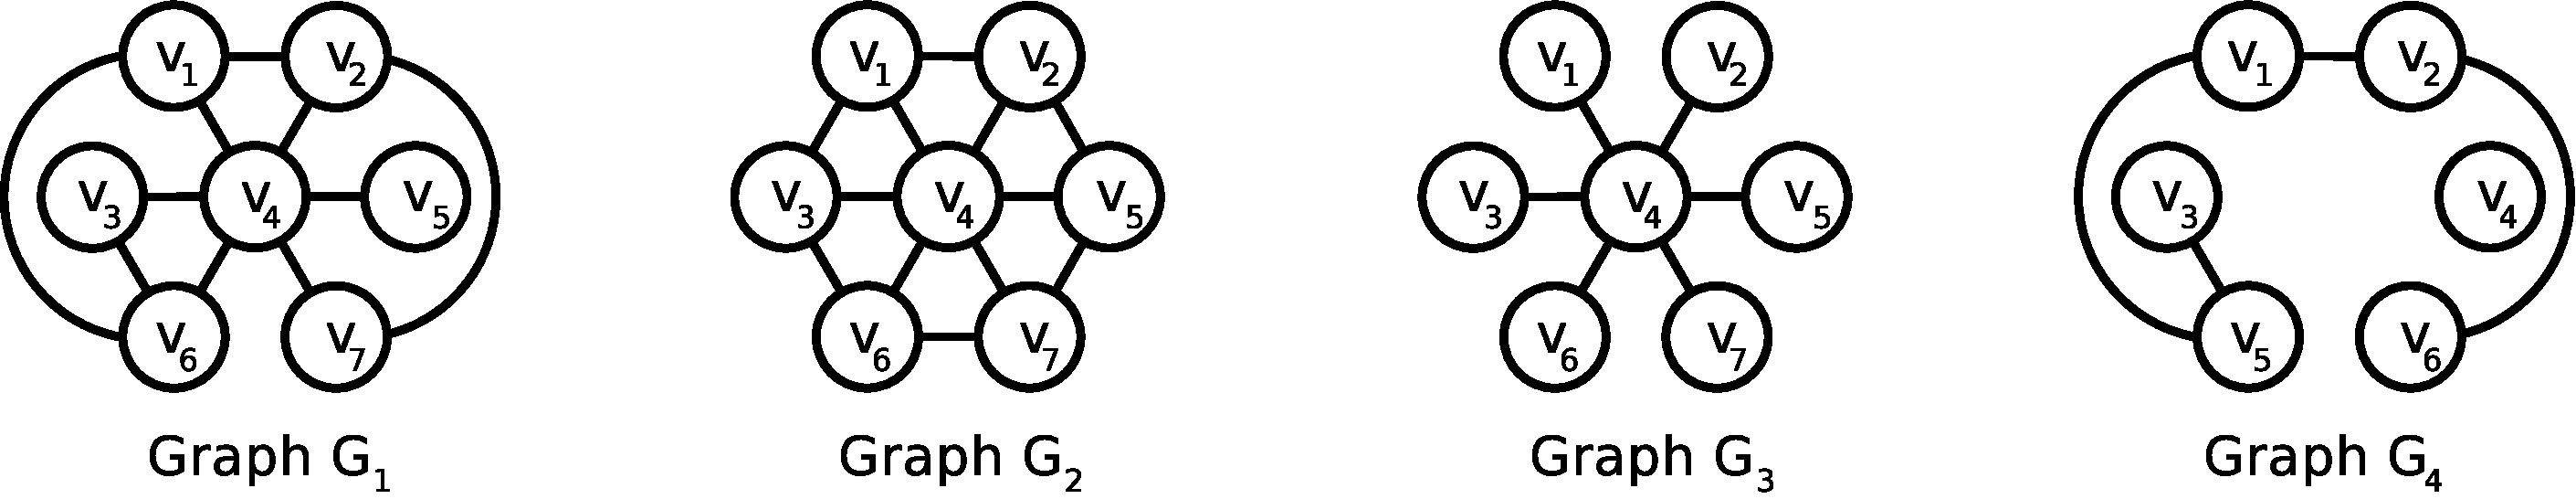
\includegraphics[width=430pt]{bilder/bsp2.pdf}
	\caption{Vier Beispielgraphen}
  	 \end{figure}
  	 
Der Graph $G_3$ ist ein Teilgraph von den Graphen $G_1$ und $G_2$. Der Graph $G_4$ ist ein induzierter Teilgraph von dem Graphen $G_1$, welcher durch das Löschen des Knotens $v_4$ entsteht. Durch das Löschen von den Kanten $\{v_1,v_3\}$,$\{v_2,v_5\}$,$\{v_5,v_7\}$ und $\{v_6,v_7\}$ in dem Graphen $G_2$ entsteht ein Teilgraph von dem Graphen $G_1$.
\end{bsp}

Ein \emph{Weg} $p$ in $G$ von Knoten $u$ nach Knoten $w$ ist eine Folge von Knoten $$p=(v_1,\ldots,v_j)$$ mit $v_1=u$ und $v_j=w$ für $1<j$ und $\{v_{i-1},v_i\}\in E$ für $1 <i \leq j$.\\Der Knoten $u$ wir als Startknoten bezeichnet und der Knoten $w$ als Endknoten.\\Einen Weg $p$ nennt man \emph{einfach}, wenn alle Knoten $v_1,\ldots,v_j$ verschieden sind. Die \emph{Länge} eines Weges $p$ von Knoten $u$ nach Knoten $w$ entspricht der Anzahl seiner Kanten.\\Die \emph{kürzeste Weglänge} $kw(u, v)$ von einem Knoten $u$ zu einem Knoten $v$ ist die minimale Länge aller Wege von $u$ nach $v$, falls mindestens ein solcher Weg existiert, ansonsten ist die kürzeste Weglänge $\infty$.\\Die \emph{Distanz} $dist_G(u,w)$ zweier Knoten $u,w$ eines Graphen $G$ ist die Länge des kürzesten Weges in $G$ zwischen $u$ und $w$. Der \emph{Durchmesser} $diam(G)$ eines Graphen ist die maximale Distanz aller Knotenpaare aus $G$.\\
Zwei Knoten $a, b$ eines Graphen $G$ heißen verbunden in $G$, wenn $a = b$ ist oder es einen Weg in $G$ von $a$ nach $b$ gibt.\\Sind je zwei Knoten von $G$ verbindbar, so heißt $G$ zusammenhängend.\\Gibt es zwischen jedem Knotenpaar zwei (bzw. $k$) knotendisjunkte Wege, so bezeichnet man den Graphen als zweifach ($k$-fach) zusammenhängend.\\Zwei Wege sind knotendisjunkt sofern alle Knoten auf diesen Weg, ausgenommen Start und Endknoten paarweise verschieden sind. Eine $k$-fache Zusammenhangskomponente von $G$ ist ein maximaler (bzgl. der Knotenmenge) $k$-fach zusammenhängender, induzierter Teilgraph von $G$.\newline \newline
\begin{floatingfigure}[l]{200pt}
\centering
\includegraphics*[width = 200pt]{bilder/bifurkator.pdf}
\caption{Beispiel für einen Bifurkator}
\label{bild:bifurkator}
\end{floatingfigure}  	 
\vspace{-2mm}
Sei ein Graph $G=(V,E)$ gegeben. Für die Knoten $z,x$ und $y$ besteht die Menge $B$ aus allen Knoten die gleichzeitig auf einem kürzesten Weg von $z$ zu $x$ und auf einem kürzesten Weg von $z$ zu $y$ liegen. Ein Knoten $v$ aus der Menge $B$ mit maximaler Distanz zum Knoten $z$ wird als ein \emph{Bifurkator} von $z, x, y$ bezeichnet.\\
Sind zwei Knoten $u,v$ durch die Entfernung eines Trennungsknotens$x$ in zwei unterschiedlichen Teilgraphen, so liegt der Knoten $x$ auf jedem Wege von $u$ nach $v$.
\todo[inline]{def: Trennungsknoten, Kontraktion} 

\todo{NP-Vollständigkeit}
\newpage
\subsection{Spezielle Graphklassen}
Eine Graphklasse ist eine aus Graphen bestehende Menge. Viele Graphklassen entstehen durch Einschränkungen der allgemeinen Graphdefinition. Es folgt eine Auflistung unterschiedlicher Graphklassen, die in dieser Arbeit angesprochen werden.
\begin{defi}{\textbf{(Weg $P_n$)}}\\
\emph{Ein Graph der aus einem Weg (Pfad) der Länge $n$ besteht, wird als $P_n$ bezeichnet.} \end{defi}

\begin{defi}{\textbf{(Kreis $C_n$)}}\\
\emph{Ein Graph der aus einem Kreis der Länge $n$ besteht, wird als $C_n$ bezeichnet $(n \geq 3)$.} \end{defi}

\begin{defi}{\textbf{(Vollständiger Graph $K_n$)}}\\
\emph{Ein Graph heißt vollständig und wird als $K_n$ bezeichnet, wenn je zwei verschiedene der $n$ Knoten des Graphen durch eine Kante verbunden sind.} 
\end{defi}


\begin{defi}{\textbf{(Vollständig bipartiter Graph $K_{n,m}$)}}\\
\emph{Ein Graph $G$ ist bipartite sofern seine Knotenmenge in zwei disjunkte Mengen $V_1$ und $V_2$ aufgeteilt werden kann, so dass für jede Kante $\{u,v\}$ in $G$ gilt: $$(u \in V_1 \wedge v \in V_2)\vee (v \in V_1 \wedge u \in V_2)$$Sind je zwei Knoten aus $V_1$ mit $|V_1|=n$ und $V_2$ mit $|V_2|=m$ adjazent, so wird der Graph als vollständig bipartiter Graph $K_{n,m}$ bezeichnet. } \end{defi}


\begin{defi}{\textbf{(Baum $T_n$)}}\\
\emph{Ein kreisfreier und zusammenhängender Graph mit $n$ Knoten wird als Baum bezeichnet und mit $T_n$ notiert. Dabei wird jeder Knoten $v$ mit $deg(v)=1$ als Blatt bezeichnet. Die anderen Knoten werden innere Knoten genannt.} \end{defi}


\begin{defi}{\textbf{(Gitter $G_{n,m}$)}}\\
\emph{Für $m,n \geq 0$ ist das $G_{n,m}$ gefiniert durch $$G_{n,m}=(\{1,\ldots,n\}\times\{1,\ldots ,m\},\{\{(i,j),(i',j')\}||i-i'|+|j-j'|=1\} ),$$ dabei ist $|x|$ definiert als der Absolutbetrag der Zahl $x \in \mathbb{Z}$.\cite{exaktealgorithmenfuerschweregraphenprobleme} 
}\end{defi}


\begin{defi}{\textbf{(Rad $W_{1,n}$)}}\\
\emph{Wiren $n$ einzelne Knoten jeweils mit genau einem Knoten eines Kreises $C_n$ verbunden, so ensteht ein Rad $W_{1,n}$.} \end{defi}


\begin{defi}{\textbf{(Stern $S_{1,n}$)}}\\
\label{defstern}
\emph{Ein Baum mit einem inneren Knoten und $n$ Blättern wird als Stern $S_{1,n}$ bezeichnet.} \end{defi}

\begin{defi}{\textbf{(Planarer Graph)}}\\
\emph{Ein Graph ist planar, wenn es eine Zeichnung gibt, so dass keine Kanten sich kreuzen.} \end{defi}


\begin{defi}{\textbf{(Außenplanarer Graph)}}\\
\emph{Ein Graph ist außenplanar, wenn man einen neuen Knoten hinzufügen kann, welcher mit allen Knoten verbunden wird und es dann eine Zeichnung gibt, so dass keine Kanten sich kreuzen.} 
\end{defi}


\begin{defi}{\textbf{(Halin Graph)}}\\
\emph{Ein Graph $G = (V, E)$ heißt Halin Graph, falls $G$ aus einem planar eingebetteten Baum besteht, bei dem die Blätter mit einem Kreis verbunden sind.} 
\end{defi}
\begin{figure}[h!]
		\centering 		 
   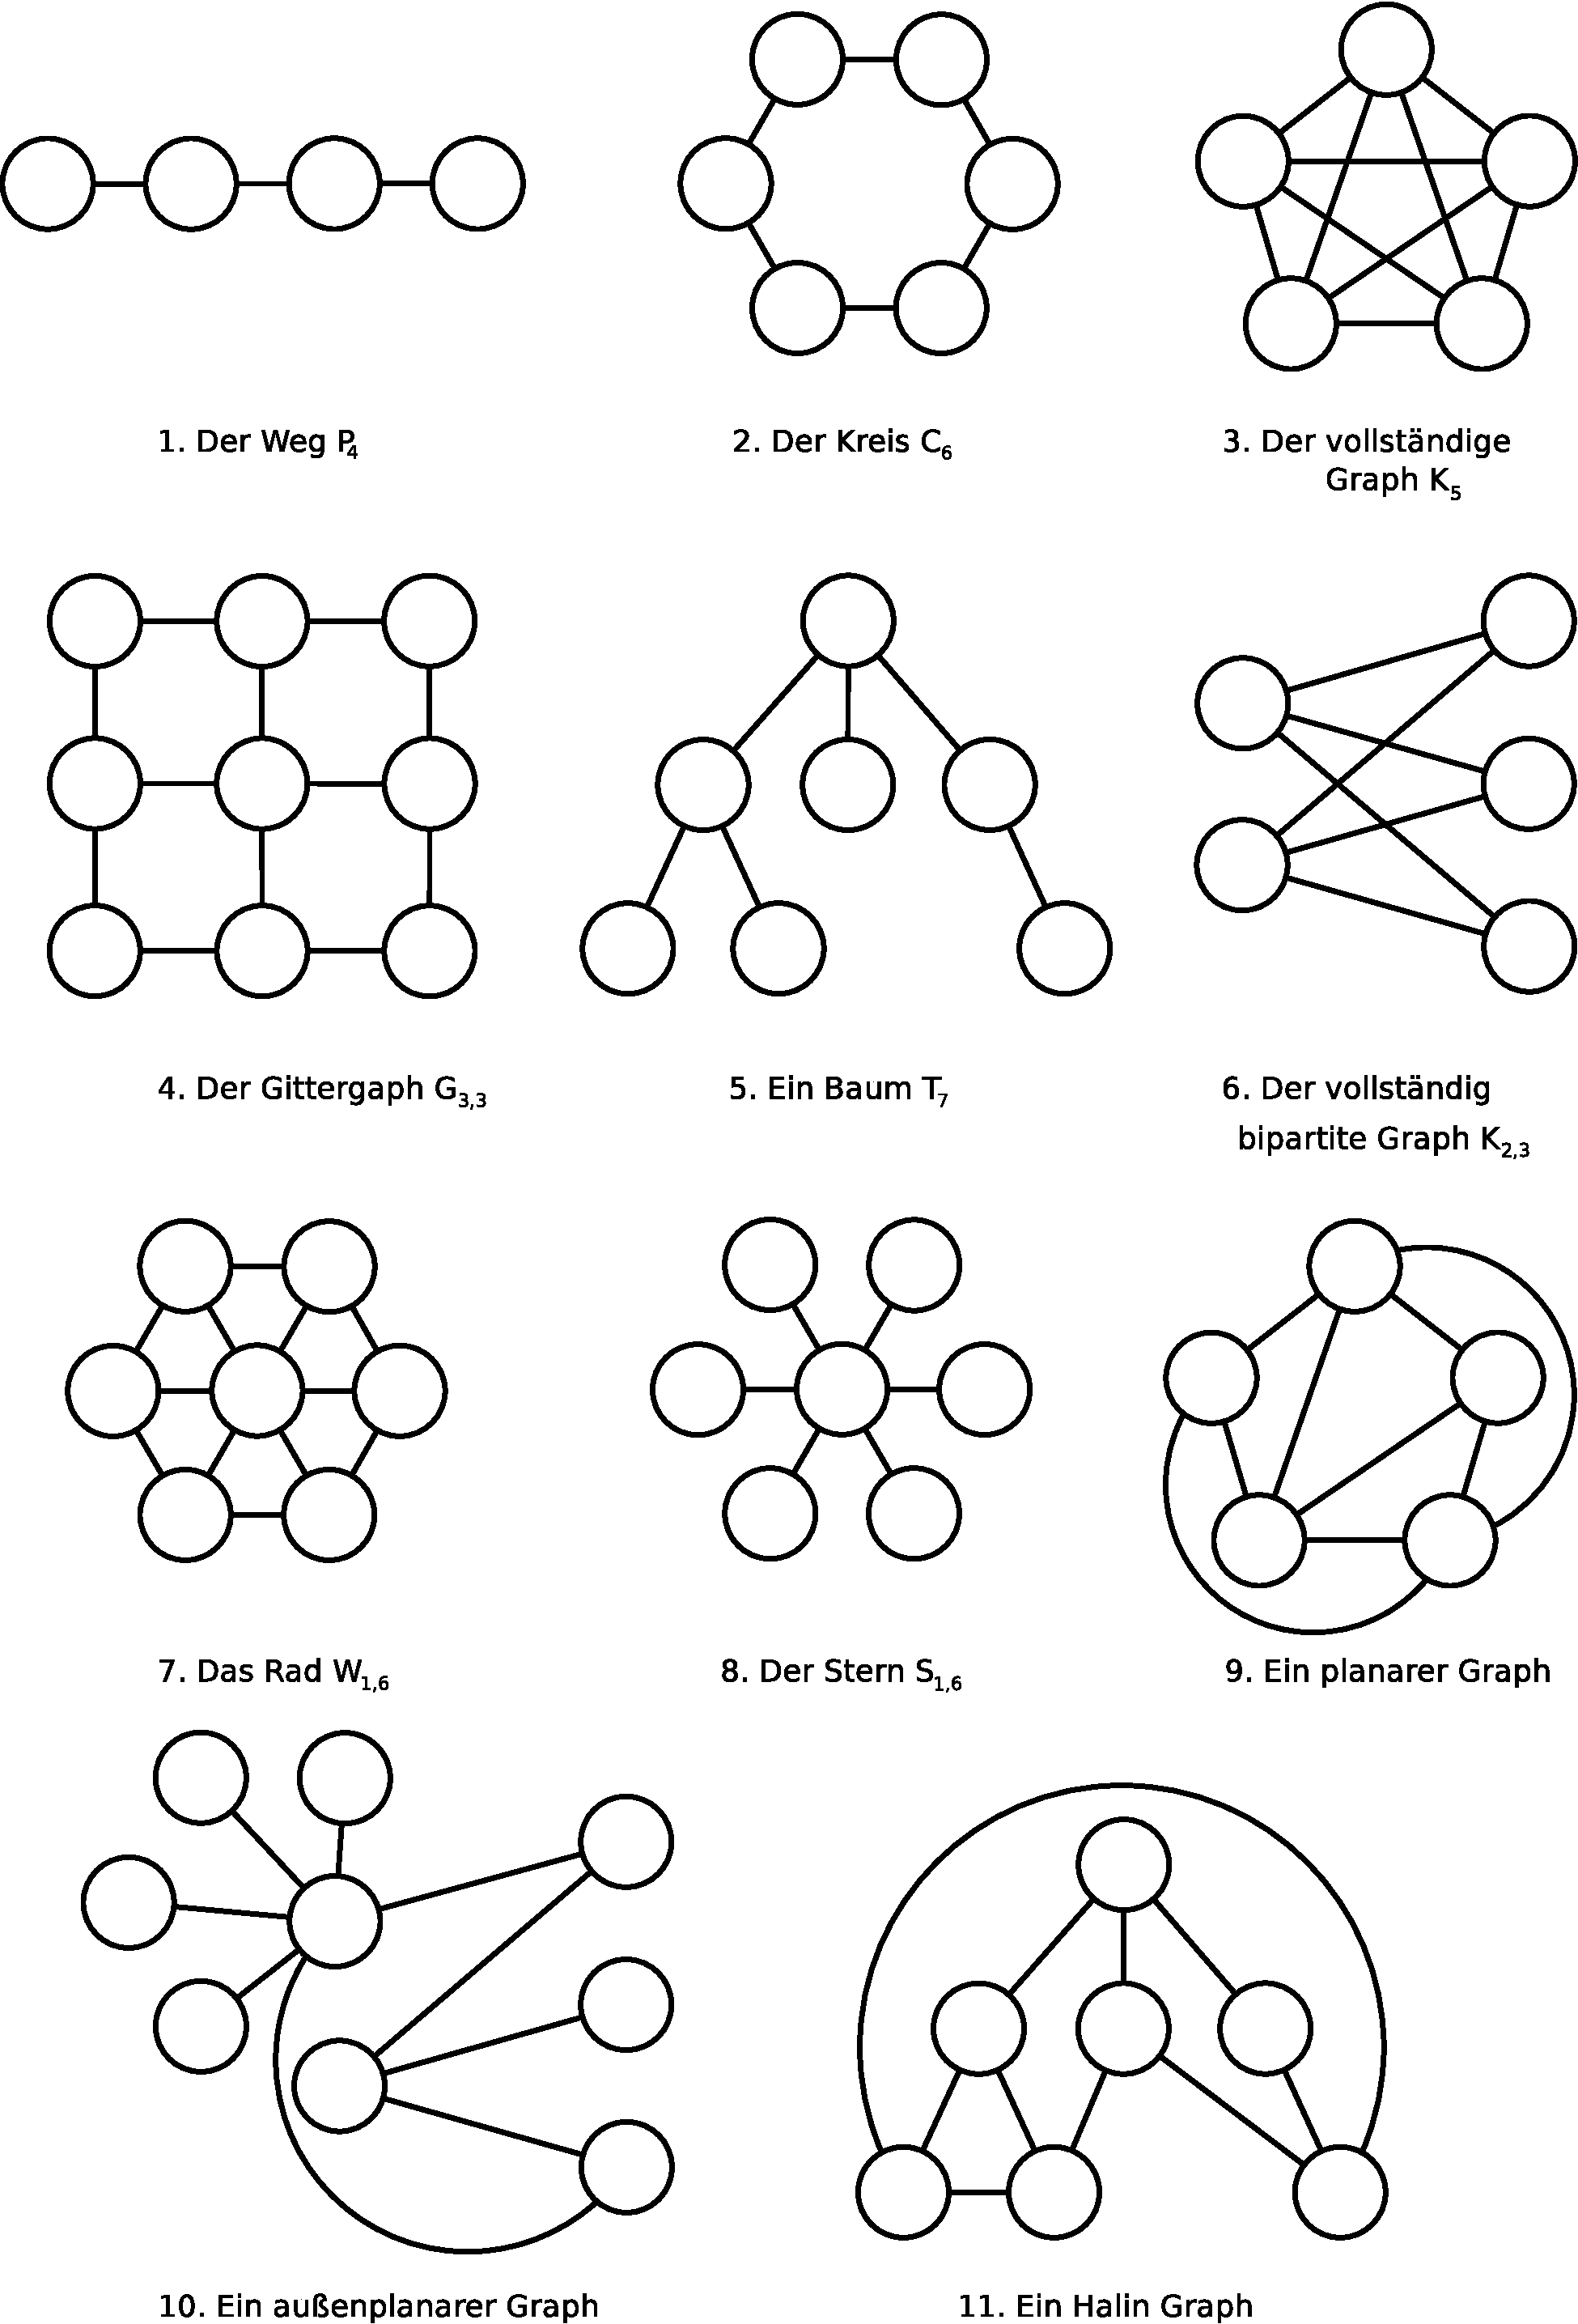
\includegraphics[width=430pt]{bilder/graphs.pdf}
	\caption{Beispiele einiger Graphklassen}
  	 \end{figure}
\clearpage
%%%%%%%%%%%%%%%%%%%%%%%%%%%%%%%%%%%%%%%%%%%%%%%%%%%%%%%%%%%%%%%%%%%%%%%%%%%%%%%%%%%%%%%%%%%%%%%%%%%%%%%%%%%%%%%%
\subsection{Metrische Dimension}
\label{MDT}
\begin{defi}{\textbf{(Metrische Dimension)}}\\
\emph{Ein Knoten $x$ eines Graphen $G$ trennt zwei Knoten $u$ und $v$ in $G$ sofern $d(x, u) \neq d(x, v)$. Eine Knotenmenge $R$ von $G$ ist eine \emph{trennende Menge} von $G$ sofern je zwei unterschiedliche Knoten in $G$ durch mindestens einen Knoten in $R$ getrennt werden. Eine \emph{Metrische Basis} von $G$ ist eine trennende Menge mit minimaler Kardinalität, welche nicht eindeutig sein muss\todo{Gibt es eindeutige MB für $|V|>1$}. Die Metrische Dimension $\beta(G)$ von $G$ ist die Kardinalität  einer Basis \cite{zzzz}. Gegeben seien eine endliche metrische Basis und eine Anordnung \todo{$R_n = \{r_1 , \ldots , r_n \} \subseteq V (G)$} und ein Knoten $v \in V (G)$, damit wird $(d(v, r_1 ), \ldots , d(v, r_n ))$ als der Vektor der \emph{Metrischen Koordinaten} von $v$ bezeichnet.} 
\end{defi}
\begin{bsp}
\end{bsp}
\textbf{Ähnliche Begriffe}\\
Neben der metrischen Dimension gibt es andere ähnliche auf Graphen definierte Probleme, die leicht in Zusammenhang mit dieser gebracht werden können.
\todo{dominating set,upper dimension, max metr. dimension u.s.w.}
%%%%%%%%%%%%%%%%%%%%%%%%%%%%%%%%%%%%%%%%%%%%%%%%%%%%%%%%%%%%%%%%%%%%%%%%%%%%%%%%%%%%%%%%%%%%%%%%%%%%%%%%%%%%%%%%
\subsection{Bekannte Resultate zur metrischen Dimension}
\begin{lem}
\label{path}
Die Metrische Dimension eines Graphens $G$ ist genau dann eins wenn der Graph $G$ ein Weg ist.\cite{landmarks} 
\end{lem}
\begin{lem}
Die Metrische Dimension eines Baumes $T$, welcher kein Weg ist, lässt sich berechnen durch $\Sigma_{v \in V:L_v >1} (l_v-1)$. Dabei ist $l_v$ die Anzahl der Brücken welche Wege sind am Knoten $v$.\cite{landmarks}
\end{lem}
\begin{lem} 
Ein $d$-dimensionales Gitter $G_d$ hat $\beta(G_d)=d$ für $d \geq 2$.(\cite{landmarks} und als falsch erklärt in \cite{somefamiliesofgraphs})
\end{lem}
  \begin{table}[htb]
     \centering
     \begin{tabularx}{\textwidth}{|>{\centering}m{4cm}|c*{5}{|>{\centering\arraybackslash}X}|}
     	\hline  
       \parbox[c][5em][c]{0pt}{~}Graphklasse $G$ & $C_n$&$K_n$& $S_{1,n}$&$W_{1,n}$ für $n \in \{3,6\}$&$W_{1,n}$ sonst \\[2em]
		\hline       
       \parbox[c][5em][c]{0pt}{~}Metr. Dimension $\beta(G)$& $2$       &$n-1$& $n-1$  &$3$  &$\lfloor \dfrac{2n+2}{5} \rfloor$        \\[2em]
       	\hline  
     \end{tabularx}
 
     \caption{Metrische Dimension einiger Graphklassen}
     \label{tbl:Metrische Dimension einiger Graphklassen}
     % Verweis im Text mittels \ref{tbl:Metrische Dimension einiger Graphklassen}
   \end{table}
\begin{comment}
\begin{lem}
Ein Kreis $C_n$ der Ordnung $n$ hat $\beta(C_n)=2$.
\end{lem}
\begin{lem}
\label{stern}
Ein Stern $S_{1,n}$ hat $\beta(S_{1,n})=n-1$.
\end{lem}
\begin{lem}
Ein vollständiger Graph $K_n$ hat $\beta(K_n)=n-1$.
\end{lem}
\begin{lem}
Ein Rad $W_{1,n}$ hat $\beta(W_{1,n})= \lfloor \dfrac{2n+2}{5} \rfloor$ für $n \notin \{3,6\}$ und $\beta(W_{1,n})=3$ für $n \in \{3,6\}$.
\end{lem}
\end{comment}
\begin{lem}
Ein Graph $G$ mit $\beta(G) = k$ kann keinen $K_{2k+1}$ als Teilgraph beiinhalten.\cite{landmarks}
\end{lem}
\begin{lem}
Sei $G = (V, E)$ ein Graph mit metrischen Dimension zwei, dann gilt folgendes:\cite{landmarks}
\begin{enumerate}
\item Der $K_{5}$, sowie der $K_{3,3}$ sind keine Teilgraphen von $G$.
%\item Ist $n \geq 3$ so kann der Graph $G$ ein Kreis $C_n$ sein.
%\item Der Graph $W_{1,5}$ und $W_{1,6}$ haben metrische Dimension zwei.FFFFFFFFFFFF!!!!!!!!!!!!!!!!!!!!!
\item Es gilt $\beta(P_m \square P_n)=2$. (2-dimensionales Gitter $n \times m$)
\end{enumerate}
\end{lem}

\begin{lem}
Sei $G = (V, E)$ ein Graph mit metrischer Dimension zwei und sei $\{a, b\} \subset V$ eine metrische Basis von $G$. Dann gilt folgendes:\cite{landmarks}
\begin{enumerate}
\item Es existiert ein eindeutiger kürzester Weg $P$ zwischen $a$ und $b$.
\item Der Grad von $a$ und $b$ ist höchstens drei.
\item Jeder anderen Knoten auf dem Weg $P$ hat höchstens den Grad fünf.
\end{enumerate}
\end{lem}
\begin{lem}
Sei $G = (V, E)$ ein Graph mit $n$ Knoten und metrischer Dimension $n-2$, dann ist der Graph eines der folgenden:\cite{landmarks}
\begin{enumerate}
\item Der $K_{r,s}$ mit $r,s \geq 1$.
\item Der $K_{r}+ \overline{K_s}$ mit $r,s \geq 1$.
\item oder der $K_{r,s}$ mit $r,s \geq 1$.
\end{enumerate}
\end{lem}
\begin{lem}
Sei ein außenplanarer Graph $G=(V,E)$ gegeben. Dann kann $\beta(G)$ in Polynomialzeit berechnet werden.\cite{onthecomplexity}
\end{lem}
\textbf{NP-Vollständigkeitsresultate}
\todo{problem definieren entschedungsproblem}
\begin{lem}
Sei ein beliebiger Graph $G=(V,E)$ gegeben. Das Minimurungsproblem für das Finden von $\beta(G)$ ist NP-vollständig.\cite{onthecomplexity}
\end{lem}

\begin{lem}
Sei ein planarer Graph $G=(V,E)$ gegeben. Das Minimurungsproblem für das Finden von $\beta(G)$ ist NP-vollständig.\cite{onthecomplexity}
\end{lem}

\begin{lem}
Sei ein bipartiter Graph $G=(V,E)$ gegeben. Das Minimurungsproblem für das Finden von $\beta(G)$ ist NP-vollständig.\cite{anefficientrepresentationofbenesnetworksanditsapplications}
\end{lem}

\textbf{Approximierbarkeit der metrischen Dimension}
\begin{lem}
Sei ein beliebiger Graph $G=(V,E)$ mit $n$ Knoten gegeben. Dann kann $\beta(G)$ approximiert werden mit dem Faktor von $O(log\:n)$ in Polynomialzeit.\cite{landmarks}
\end{lem}
%%%%%%%%%%%%%%%%%%%%%%%%%%%%%%%%%%%%%%%%%%%%%%%%%%%%%%%%%%%%%%%%%%%%%%%%%%%%%%%%%%%%%%%%%%%%%%%%%%%%%%%%%%%%%%%%
\subsection{Metrische Dimension von zusammengestellten Graphen}
\begin{defi}{\textbf{(Vereinigung)}}\\
\emph{Gegeben seien zwei Graphen $G_1=(V_1,E_1)$ und $G_2=(V_2,E_2)$. Aus der Vereinigung $G_{1+2}=G_1+G_2$ entsteht der Graph mit der Knotenmenge $V_{1+2}=V_1 \cup V_2$ und der Kantenmenge $E_{1+2}= E_1 \cup E_2 \cup \{\{v_1,v_2\}| v_1 \in V_1 \wedge v_2 \in V_2\}$.} 
\end{defi}

\begin{defi}{\textbf{(Kartesisches Produkt)}}\\
\emph{Gegeben seien zwei Graphen $G_1=(V_1,E_1)$ und $G_2=(V_2,E_2)$. Aus dem kartesischen Produkt $G_{1\square 2}=G_1 \square G_2$ entsteht der Graph mit der Knotenmenge $V_{1 \square 2}=V_1 \times V_2$ und der Kantenmenge $E_{1\square 2}= \{\{(x_1,x_2),(y_1,y_2)\}| (x_1=y_1 \wedge \{x_2,y_2\} \in E_2)\vee (x_2=y_2 \wedge \{x_1,y_1\} \in E_1)\}$.} 
\end{defi}

\begin{defi}{\textbf{($r$-fache Verschmelzung)}}\\
\emph{Gegeben seien zwei Graphen $G_1=(V_1,E_1)$ und $G_2=(V_2,E_2)$ mit $|V_1|, |V_2| \geq r$ und zwei Teilmengen $V_{1,r} \subseteq V_1$ und $V_{2,r} \subseteq V_2$ mit $|V_{1,r}|, |V_{2,r}| = r$. Aus der $r$-fachen Verschmelzung $G_{1 \infty 2}=G_1 \infty G_2$ entsteht der Graph mit der Knotenmenge $V_{1 \infty 2}=V_1 \cup V_2\backslash V_{2,r}$ und der Kantenmenge $E_{1\infty 2}= E_1 \cup E_2$. Außerdem gilt, dass genau ein Knoten aus $V_{1,r}$ mit genau einem Knoten aus $V_{2,r}$ verschmolzen wird.} 
\end{defi}

\begin{defi}{\textbf{($r$-fache Vereinigung)}}\\
\emph{Gegeben seien zwei Graphen $G_1=(V_1,E_1)$ und $G_2=(V_2,E_2)$ mit $|V_1|, |V_2| \geq r$ und zwei Teilmengen $V_{1,r} \subseteq V_1$ und $V_{2,r} \subseteq V_2$ mit $|V_{1,r}|, |V_{2,r}| = r$. 
Aus der $r$-fachen Vereinigung $G_{1 \leftrightarrow 2}= G_1 \leftrightarrow G_2$ entsteht der Graph mit der Knotenmenge $V_{1 \leftrightarrow 2}=V_1 \cup V_2$ und der Kantenmenge $E_{1\leftrightarrow 2}= E_1 \cup E_2 \cup E_{\leftrightarrow }$ mit $E_{\leftrightarrow}=\{\{v_1,v_2\}| v_1 \in V_{1,r} \wedge v_2 \in V_{2,r} \}$ und dabei gilt für jedes $v_1 \in V_{1,r}$ das $|\{\{v_1,v_2\} \in E_{\leftrightarrow} \wedge  v_2 \in V_{2,r} \}|= 1$ und für jedes $v_2 \in V_{2,r}$ das $|\{\{v_1,v_2\} \in E_{\leftrightarrow} \wedge v_1 \in V_{1,r} \}|= 1$ .} 
\end{defi}
\begin{bsp} \textcolor{white}{x}
\begin{figure}[h!]
		\centering 		 
   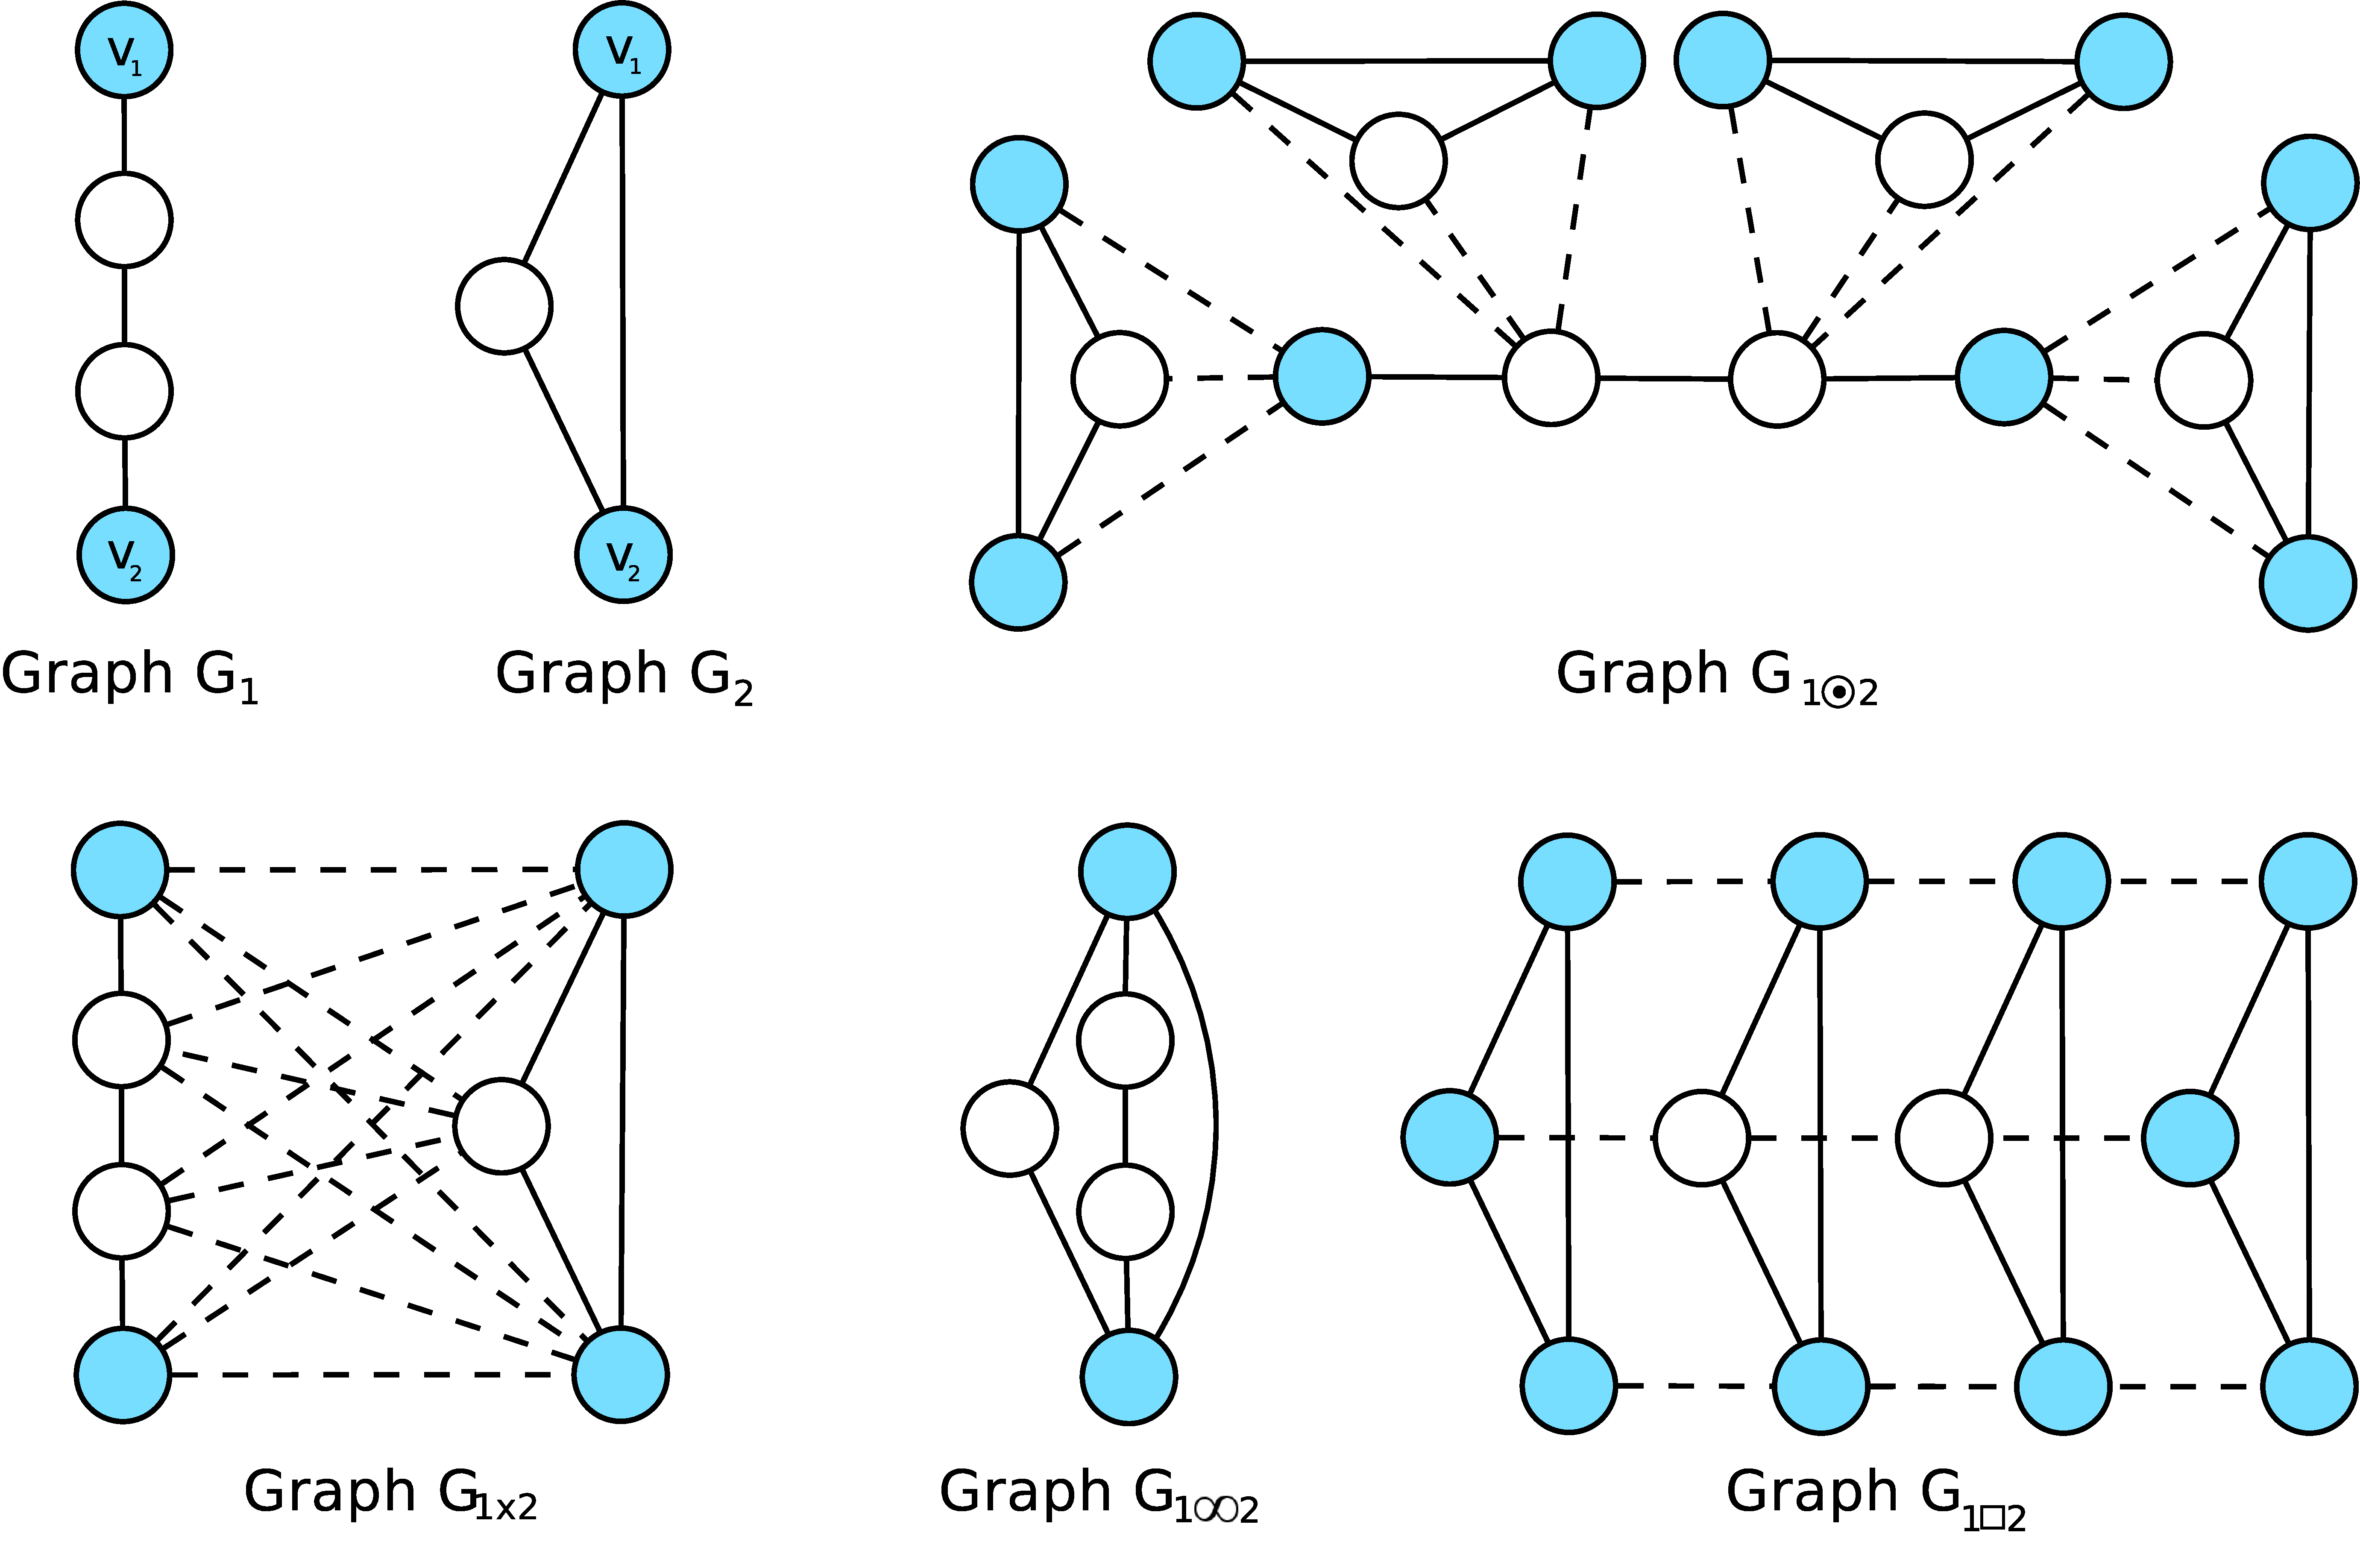
\includegraphics[width=427pt]{bilder/struktur2.pdf}
	\caption{Beispiel für Vereinigung, kartesisches Produkt,$r$-fache Vereinigung und $r$-fache Verschmelzung}
  	 \end{figure}
\end{bsp}
\newpage
\begin{lem}(Bekannte Ergebnisse für Vereinigung und für das kartesische Produkt\cite{somefamiliesofgraphs})
\begin{itemize}
\item $max\{\beta(G),\beta(H)\}\leq \beta(G\square H) \leq min\{\beta(G)+|H|,\beta(H)+|G|\}-1$
\item $2 \leq \beta(G) \leq \beta(H) \leq \beta(G\square H) \leq min\{\beta(G)+|H|,\beta(H)+|G|\}-2$
\item $\beta(G)+\beta(H) \leq \beta(G+H)$
\item $\beta(G)\leq \beta(G\square K_2) \leq \beta(G)+1$
\item $\beta(G)\leq \beta(G\square P_n) \leq \beta(G)+1$
\item $\beta(G\square K_n) \leq \beta(G)+n-2$ für $n \geq 3$
\item $\beta(G\square C_n) \leq \beta(G)+1$ für $n$ ungerade
\item $\beta(G\square C_n) \leq \beta(G)+2$ für $n$ gerade
\item $\beta(P_m+P_n)=2$
\item $\beta(P_m+K_n)=n-1$ für $n\geq 3$
\item $\beta(P_m+C_n)=2$ für $n$ ungerade
\item $\beta(P_m+C_n)=2$ für $n$ gerade und $m \neq 1$
\item $\beta(C_m+C_n)=3$ falls $m$ oder $n$ gerade
\item $\beta(C_m+C_n)=4$ sonst
\item $\beta(K_m+C_n)=m$ falls $m=4$ und $n$ ungerade
\item $\beta(K_m+C_n)=m-1$ sonst
\end{itemize}
\end{lem}

\begin{lem}$\;\;$\\Folgende Schranken gelten für die $r$-fache Verschmelzung von Graphen mit $r \geq 4$:
$$\beta(G_1)+\beta(G_2)-2r \leq \beta(G_1 \infty G_2) \leq \beta(G_1)+\beta(G_2)+r+2 \cdot \lfloor\frac{(r-2)}{3}\rfloor+1$$
\end{lem}

\begin{proof}[Beweis:] 
Um zu zeigen, dass die Schranken strikt sind werden zwei folgende Klassen von Graphen betrachtet. Für die obere Schranke gilt:\\
Betrachte man den folgenden Graphen $G_1$ mit der metrischen Dimension $2$.
\begin{figure}[h!]
		\centering 		 

\includegraphics[width=420pt]{bilder/ver.pdf}
   \caption{Graph $G_1$ mit der metrischen Dimension $2$}
  	 \end{figure}
  	 \newpage
Um zu zeigen das $\beta(G_1)=2$ betrachte die einzelnen Komponenten des Graphen. Nach Lemma \ref{path} ist bekannt, dass die metrische Dimension eines Weges eins ist. Aufgrund der zwei Blätter am linken und rechten Rand, werden mindestens zwei Knoten in der metrischen Basis benötigt. Auf dem Weg sind zusätzlich Kreise der Größe sechs, aber die Knoten des Graphens werden ohne zusätzlich Vergrößerung der metrischen Dimension getrennt. Betrachte dazu die provisorischen Markierungen in der Abbildung \ref{bild:Kreise}.
\begin{figure}[h!]
		\centering 		 
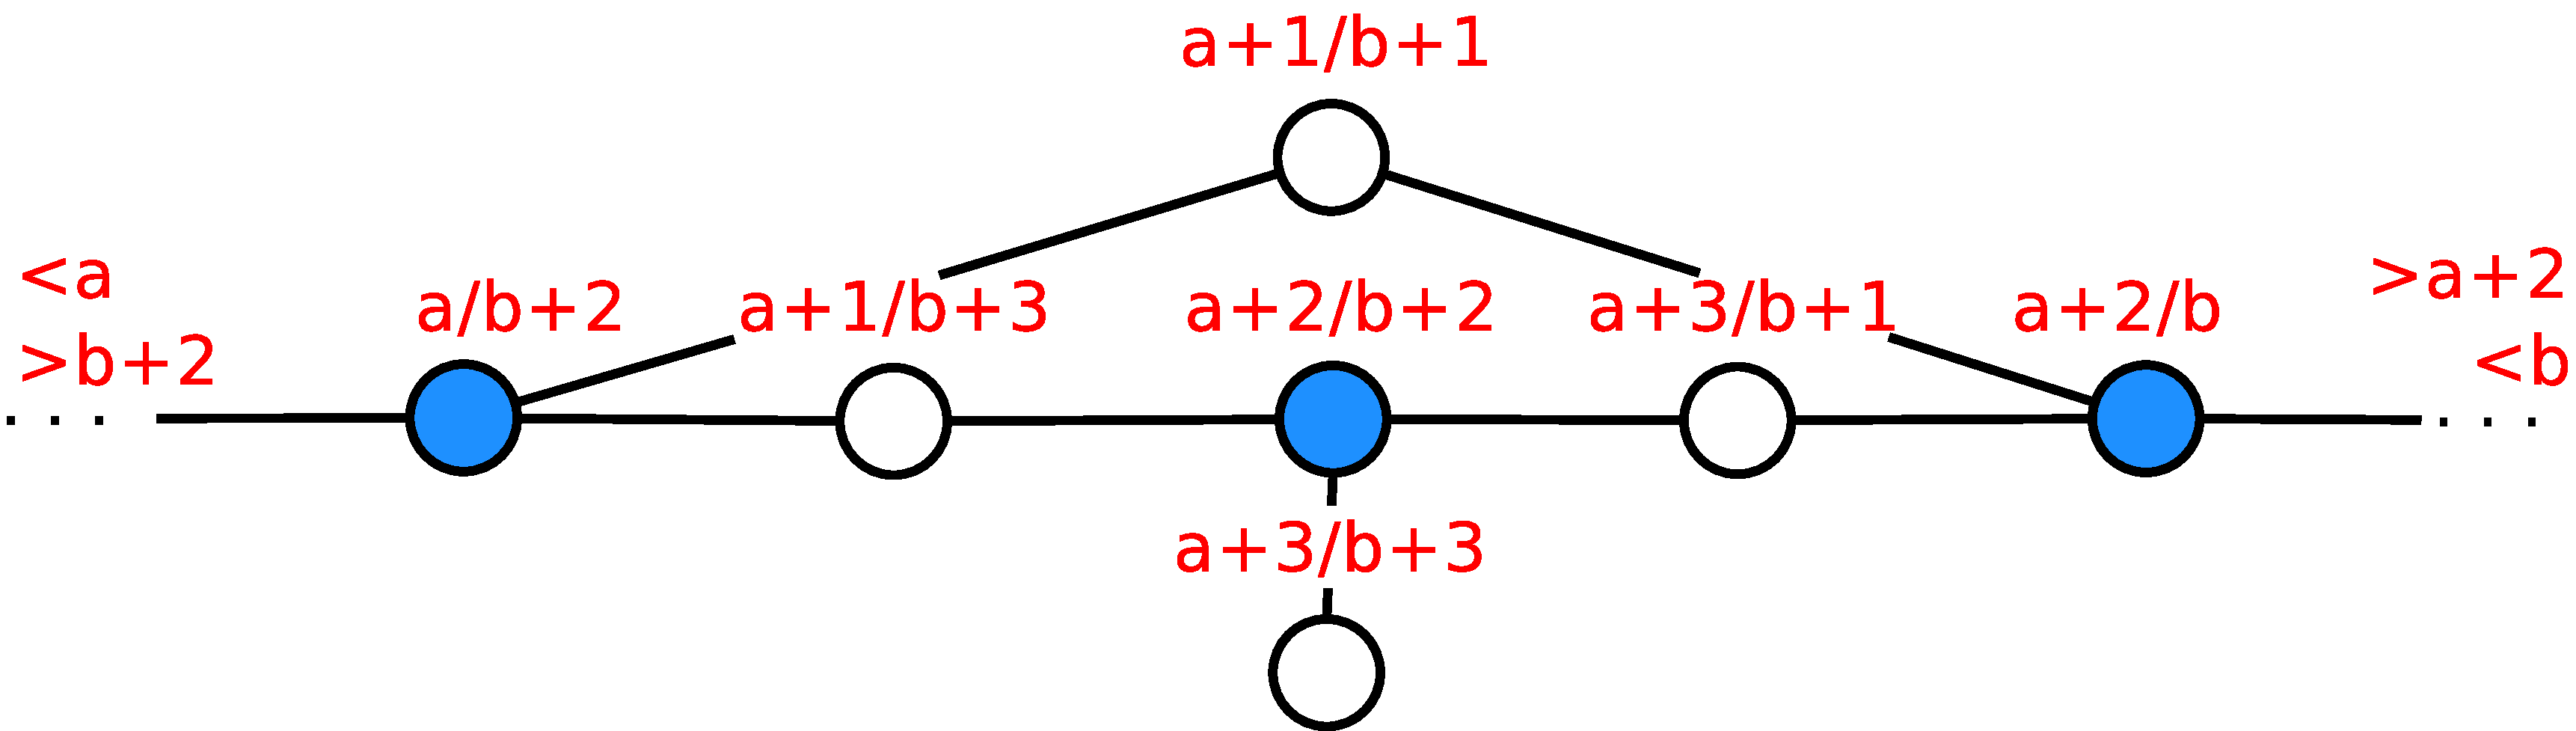
\includegraphics[width=420pt]{bilder/ver2.pdf}
   \caption{Kreise der Länge 6 in Graphen $G_1$}
   \label{bild:Kreise}
  	 \end{figure} 
  	 
Erzeuge einen äquivalenten Graphen $G_2$ mit welchem $G_1$ verschmolzen wird, so entsteht der folgenden Graph:

\begin{figure}[h!]
		\centering 		 

\includegraphics[width=420pt]{bilder/verschmolzenlandmarks.pdf}
   \caption{Graph $G_1$ und $G_2$ wurden verschmolzen}
  	 \end{figure}

Die metrische Dimension von diesem Graphen beträgt:

$$ \beta(G_1)+\beta(G_2)+2+r-1+ \lfloor(r-2)\times\frac{1}{3}\rfloor = \beta(G_1)+\beta(G_2)+r+2 \cdot \lfloor\frac{(r-2)}{3}\rfloor+1$$

\newpage

	   	 
\begin{floatingfigure}[l]{200pt}
\centering
\includegraphics*[width = 160pt]{bilder/gbspver1.pdf}
\caption{Gegenbeispiel für eine mögliche Verbesserung}
\label{bild:aussenknoten}
\end{floatingfigure}
Es nicht möglich dieses Modell durch weitere Kreise zu erweitern. Die außenliegenden Knoten, welche verschmolzen werden, können keine zusätzlichen Kreise bilden, da ein nicht getrenntes Knotenpaar entsteht. Das nichtgetrennte Knotenpaar ist rot markiert in der Abbildung \ref{bild:aussenknoten}. Außerdem muss mindestens ein Knoten, der verschnolzen wird Abstand gehalten werden, ansonsten gibt es mehrere nicht getrennte Knotenpaare, wie in der Abbildung \ref{bild:2hintereinander} dargestellt. Der Versuch weitere größere Kreise zu schaffen, scheitert schon am nächstgrößeren Beispiel, welches in der Abbildung \ref{bild:multikreise} dargestellt ist.

 
 \begin{figure}[h!]
		\centering 		 
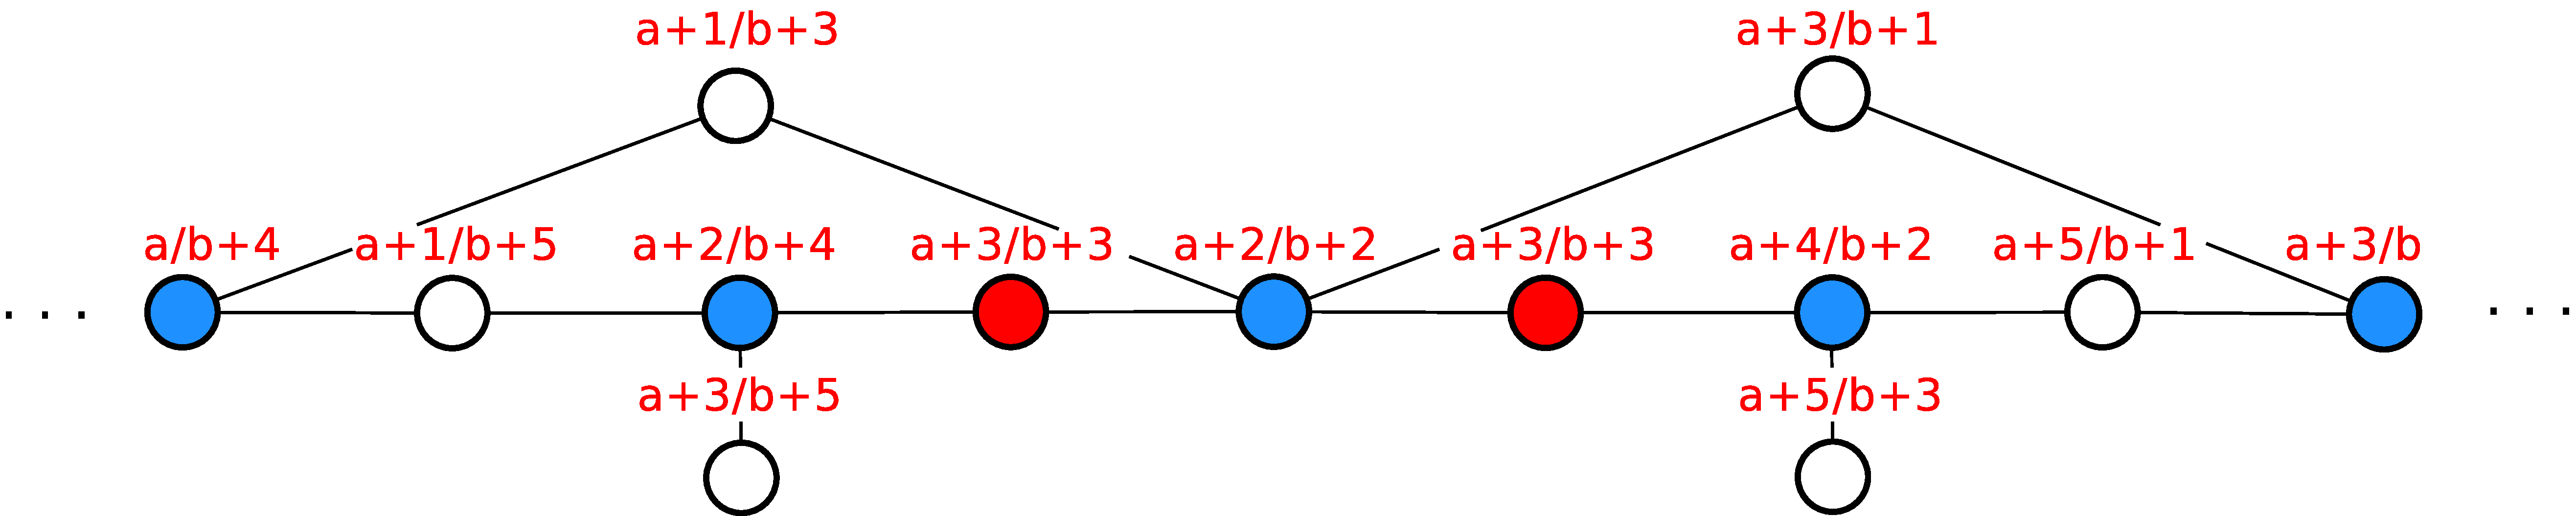
\includegraphics[width=420pt]{bilder/gbspver2.pdf}
   \caption{Gegenbeispiel für eine mögliche Verbesserung}
\label{bild:2hintereinander}  	 
  	 \end{figure}  


 \begin{figure}[h!]
		\centering 		 
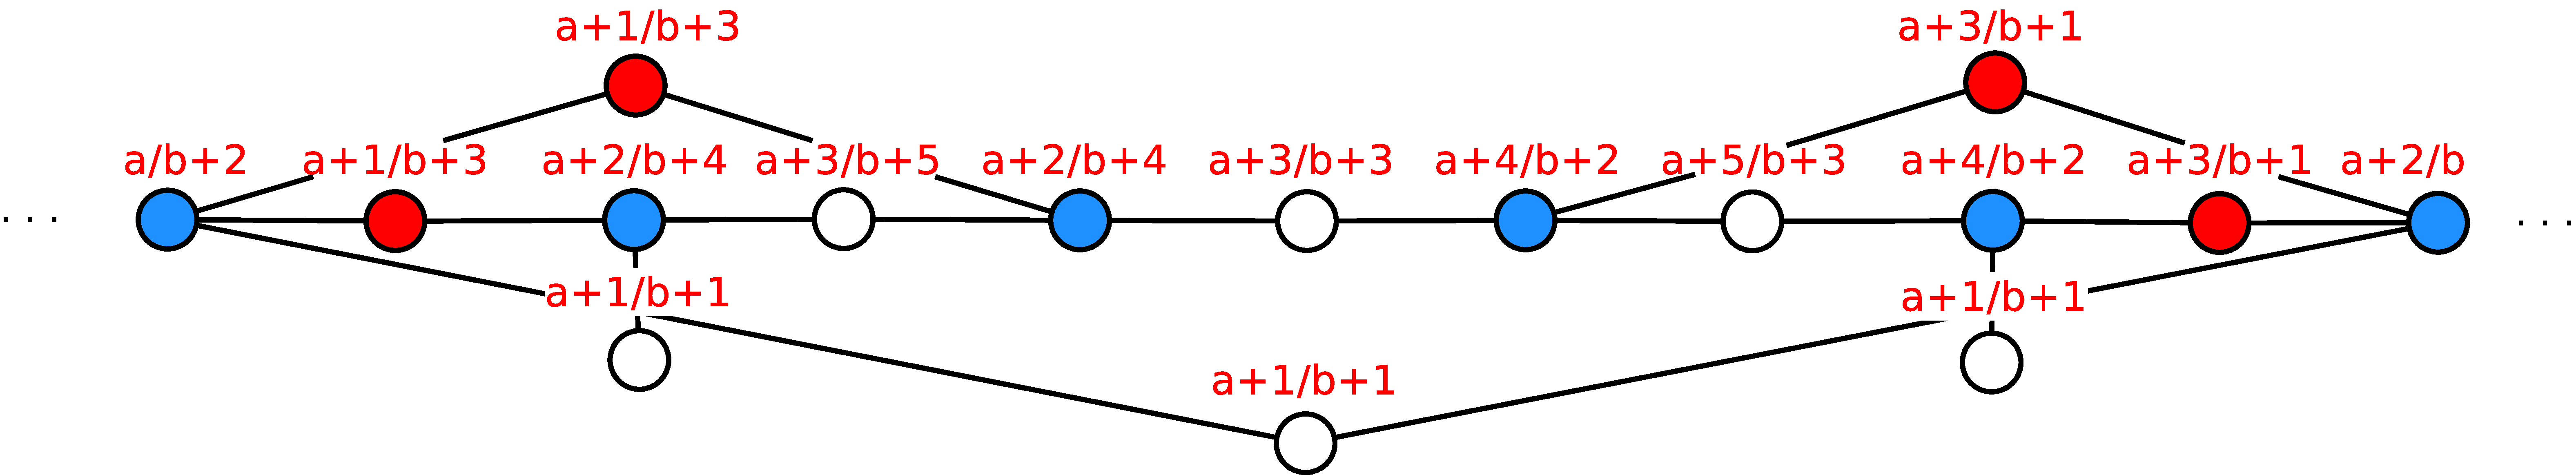
\includegraphics[width=420pt]{bilder/gbsp3.pdf}
   \caption{Gegenbeispiel für eine mögliche Verbesserung}
\label{bild:multikreise}  	 
  	 \end{figure} 
\end{proof}

\clearpage
%%%%%%%%%%%%%%%%%%%%%%%%%%%%%%%%%%%%%%%%%%%%%%%%%%%%%%%%%%%%%%%%%%%%%%%%%%%%%%%%%%%%%%%%%%%%%%%%%%%%%%%%%%%%%%%%
%%%%%%%%%%%%%%%%%%%%%%%%%%%%%%%%%%%%%%%%%%%%%%%%%%%%%%%%%%%%%%%%%%%%%%%%%%%%%%%%%%%%%%%%%%%%%%%%%%%%%%%%%%%%%%%%
%%%%%%%%%%%%%%%%%%%%%%%%%%%%%%%%%%%%%%%%%%%%%%%%%%%%%%%%%%%%%%%%%%%%%%%%%%%%%%%%%%%%%%%%%%%%%%%%%%%%%%%%%%%%%%%%
\section{Metrische Dimension dreier Graphklassen}
\subsection{Stuktur Eigenschaften}
Es erscheint einem ganz natürlich, dass durch das Entfernen von Kanten sich die metrische Dimension verringert. Nehme man zum Beispiel einen vollständigen Graphen $K_n$ und entferne solange Kanten bis der Graph zu einem einfachen Weg $P_n$ wird. Nun hat sich die metrische Dimension von $n-1$ auf $1$ verringert, also um einen Faktor von $n-1$.\\Interessant ist aber die Eigenschaft, dass durch die Entfernung von Kanten die metrische Dimension auch ansteigen kann. Der folgende Satz und Beweis zeigen, dass sich die metrische Dimension bezüglich des Löschens von Kanten bei einer Graphklasse von einem konstanten Wert um einen unbeschränkten Faktor vergrößert.
\begin{lem}
Die metrische Dimension eines Teilgraphen ist nicht durch die metrische Dimension des ursprünglichen Graphen beschränkt. (Durch das Entfernen von Kanten kann die metrische Dimension eines Graphen steigen.)
\end{lem}
\begin{proof}[Beweis:]$\;$
\begin{figure}[h!]
		\centering 		 
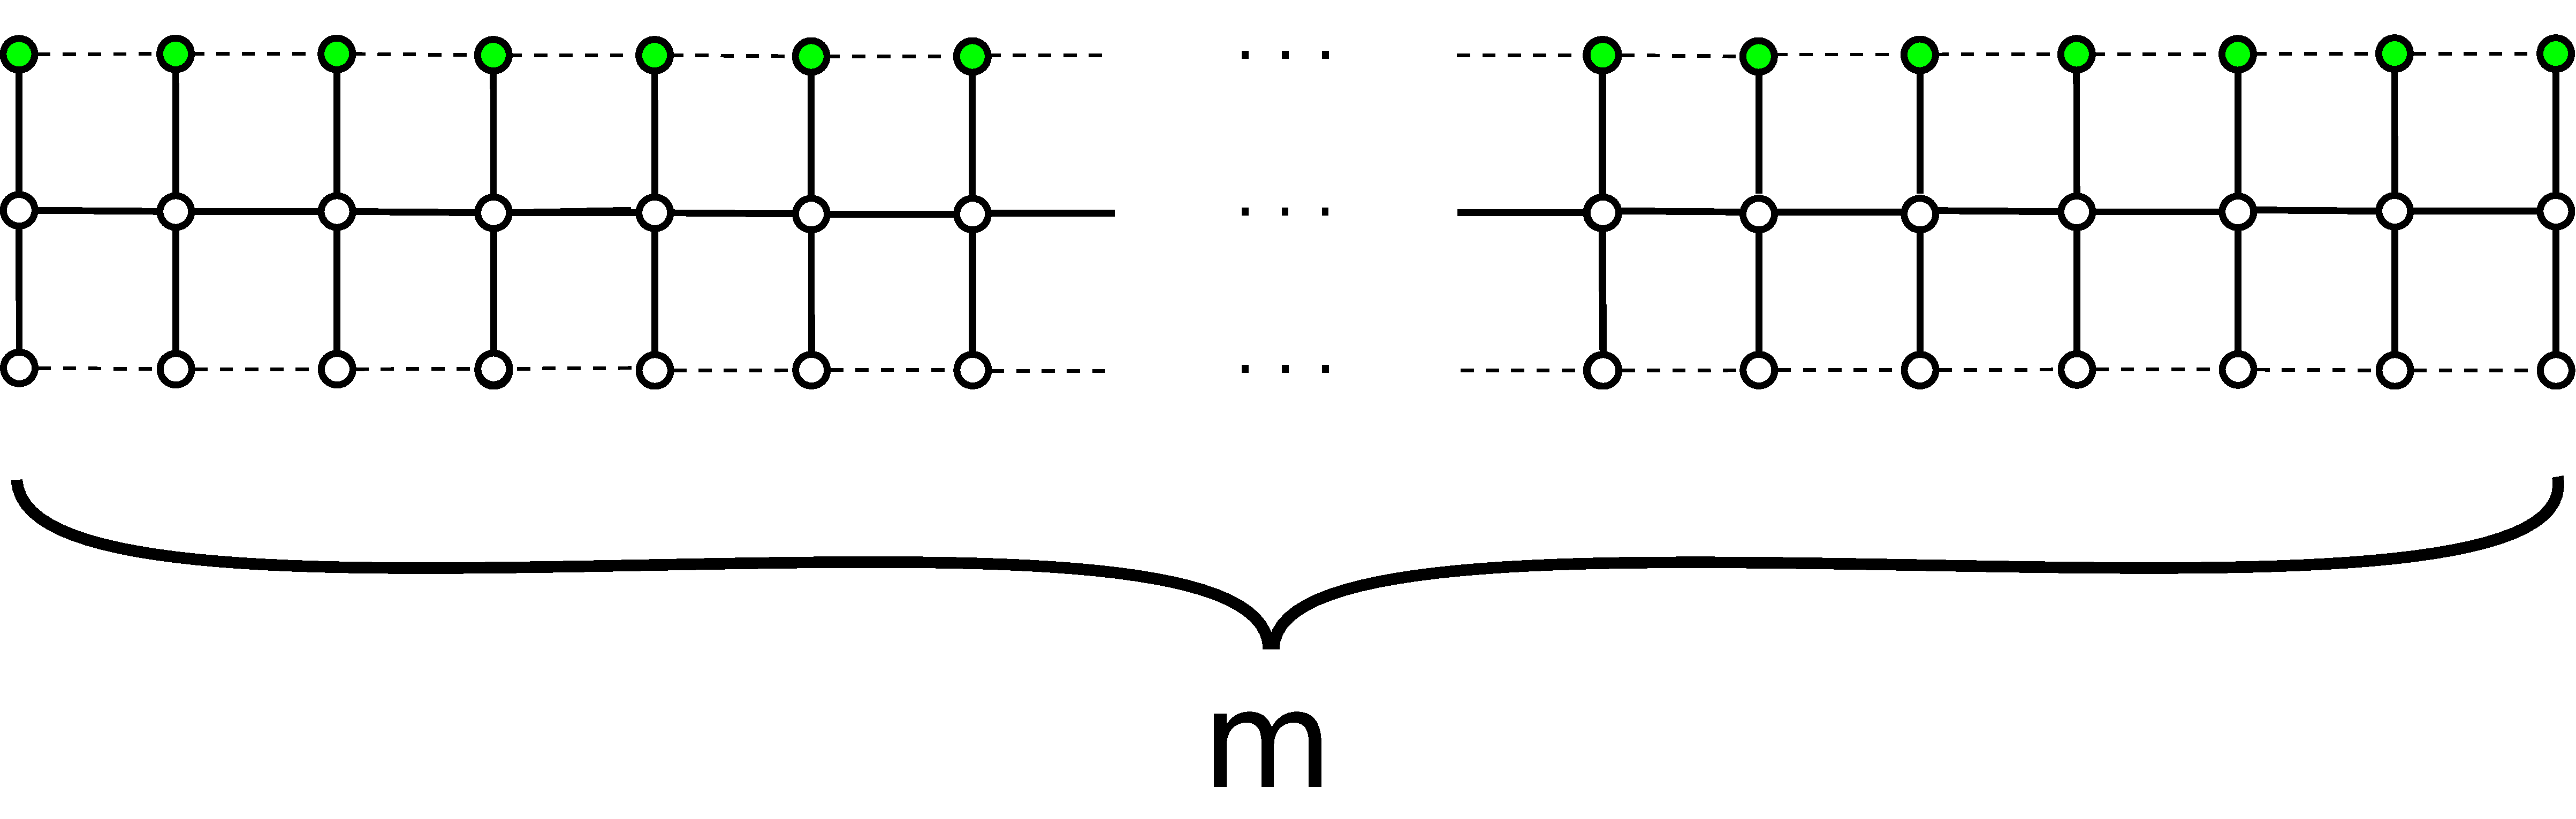
\includegraphics[width=420pt]{bilder/gitterzubaum.pdf}
   \caption{Beispiel für einen Teilgraphen mit größerer MD als der Graph selbst}
   \label{bild:Gitterbaum1}
\end{figure}
\textcolor{white}{x}\newline
Der Gittergraph $G_{3,m}$ hat nach der Tabelle \ref{tbl:Metrische Dimension einiger Graphklassen} metrische Dimension zwei. Entfernt man alle Kanten auf dem aüßeren Kreis so entsteht ein Baum $T_{3m}$ wie in Abbildung \ref{bild:Gitterbaum1} mit der metrischen Dimension $m$. Damit steigt die metrische Dimension von einem Graphen mit $n$ Knoten von zwei auf $\frac{n}{3}$.
\end{proof}
\begin{lem}
Die metrische Dimension eines induzierten Teilgraphen ist nicht durch die metrische Dimension des ursprünglichen Graphen beschränkt. (Durch das Entfernen von Knoten kann die metrische Dimension eines Graphen steigen.)
\end{lem}
\begin{proof}[Beweis:]$\;$
\begin{figure}[h!]
		\centering 		 
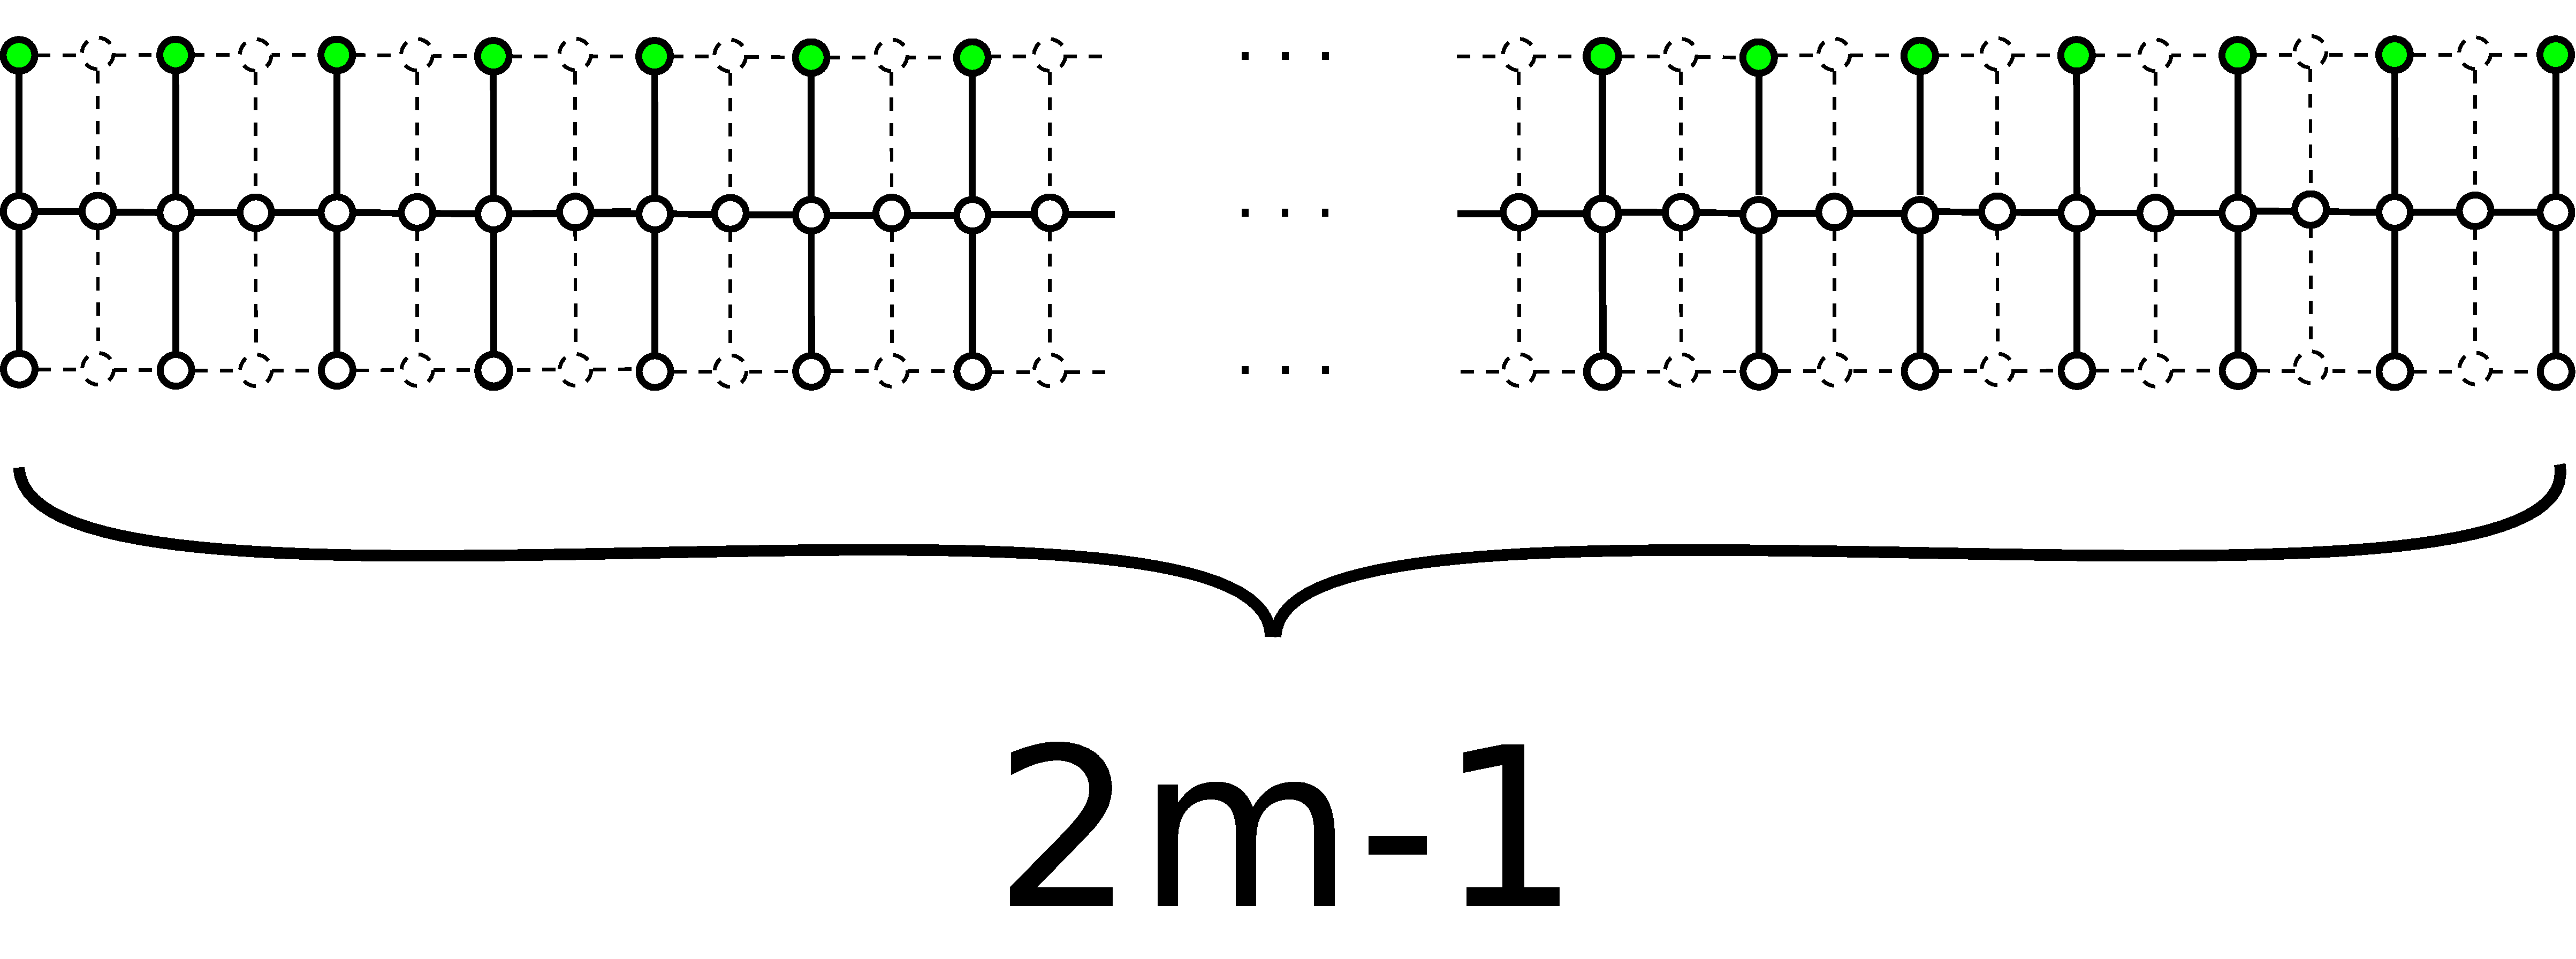
\includegraphics[width=420pt]{bilder/gitterzubaumlsch2.pdf}
   \caption{Beispiel für einen induzierten Teilgraphen mit größerer MD als der Graph selbst}
   \label{bild:Gitterbaum2}
  	 \end{figure}
\textcolor{white}{x}\newline
Der Gittergraph $G_{3,2m-1}$ hat nach der Tabelle \ref{tbl:Metrische Dimension einiger Graphklassen} metrische Dimension zwei. Entfernt man jeden zweiten Knoten auf dem aüßeren Kreis so entsteht ein Baum $T_{3m}$ wie in Abbildung \ref{bild:Gitterbaum2} mit der metrischen Dimension $m$. Damit steigt der Anteil von Knoten : Knoten in der metrischen Basis von $6m$-$3:2$ auf $3m:m$.
\end{proof}
\begin{lem}
\label{dist}
Sei $G=(V,E)$ ein gegebener Graph. Seien $u,v$ und $w$ Knoten in $G$ und sei $\{u,v\}\in E$. Sei $d$ die Länge eines kürzesten Weges von $u$ zu $w$ in $G$. Dann ist die Länge eines kürzesten Weges von $v$ zu $w$ ein Element der Menge $\{d-1,d,d+1\}$.\cite{landmarks}
\end{lem}
\begin{lem}
\label{trennungsknoten}
Sei ein beliebiger Graph $G=(V,E)$ gegeben. Seien $G_1$ und $G_2$ zwei disjunkte Teilgraphen von $G$ die durch das Löschen von einem Knoten $x$ entstehen. Jedes Knotenpaar aus $G_2$, welches von einem Knoten aus $G_1$ getrennt wird, weird auch von dem Knoten $x$ getrennt. Es gilt dasselbe für die Knotenpaare in $G_1$.
\end{lem}
\begin{comment}
\begin{lem}
Sei ein beliebiger Graph $G=(V,E)$ mit der metrischen Dimension $r$ gegeben. Sei $G*$ ein Teilgraph von $G$ mit der metrischen Dimension $k \leq r$ und der metrischen Basis $R_k$. Die Anzahl der Trennungsknoten vom Grad zwei summiert mit der Anzahl der Elemente aus der metrischen Basis von $G*$ hat mindestens die Größe der metrischen Dimension vom Teilgraphen. Der Knoten, welcher mit dem Trennungsknoten verbunden ist wird als $v_t$ bezeichnet.
\end{lem}
\begin{proof}[Beweis mittels vollständiger Induktion über die Anzahl der Trennungsknoten:]$\;$
\begin{itemize}
\item[IA:] Sei der Graph $G*$ nur über einen Knoten vom Grad zwei mit dem Restgraphen verbunden. Werden dieselben Elemente in die metrische Basis aufgenommen wie zuvor, so werden alle Knoten in $G*$ getrennt. 
Wird ein Element aus $G\setminus{G*}$ in die metrische Basis aufgenommen, so kann höchstens ein Element aus $R_k$ entfernt werden. 
\item[IV:] 
\item[IS:]
\end{itemize}
\end{proof}
\end{comment}
\begin{lem}
\label{first_theorem}
Gegeben ein Graph bestehend aus zwei Teilgraphen $G_R$ und $G_L$, welche durch genau eine Kante verbunden sind. Sofern jeder Teilgraph mind. ein Element aus der metrischen Basis beinhalten, so ist jedes Knotenpaar $x,y$ mit der Eigenschaft $x \in G_R$ und $y \in G_L$ getrennt.
\end{lem}

\begin{proof}[Beweis:]
\textcolor{white}{x}
\begin{figure}[h!]
		\centering 		 
  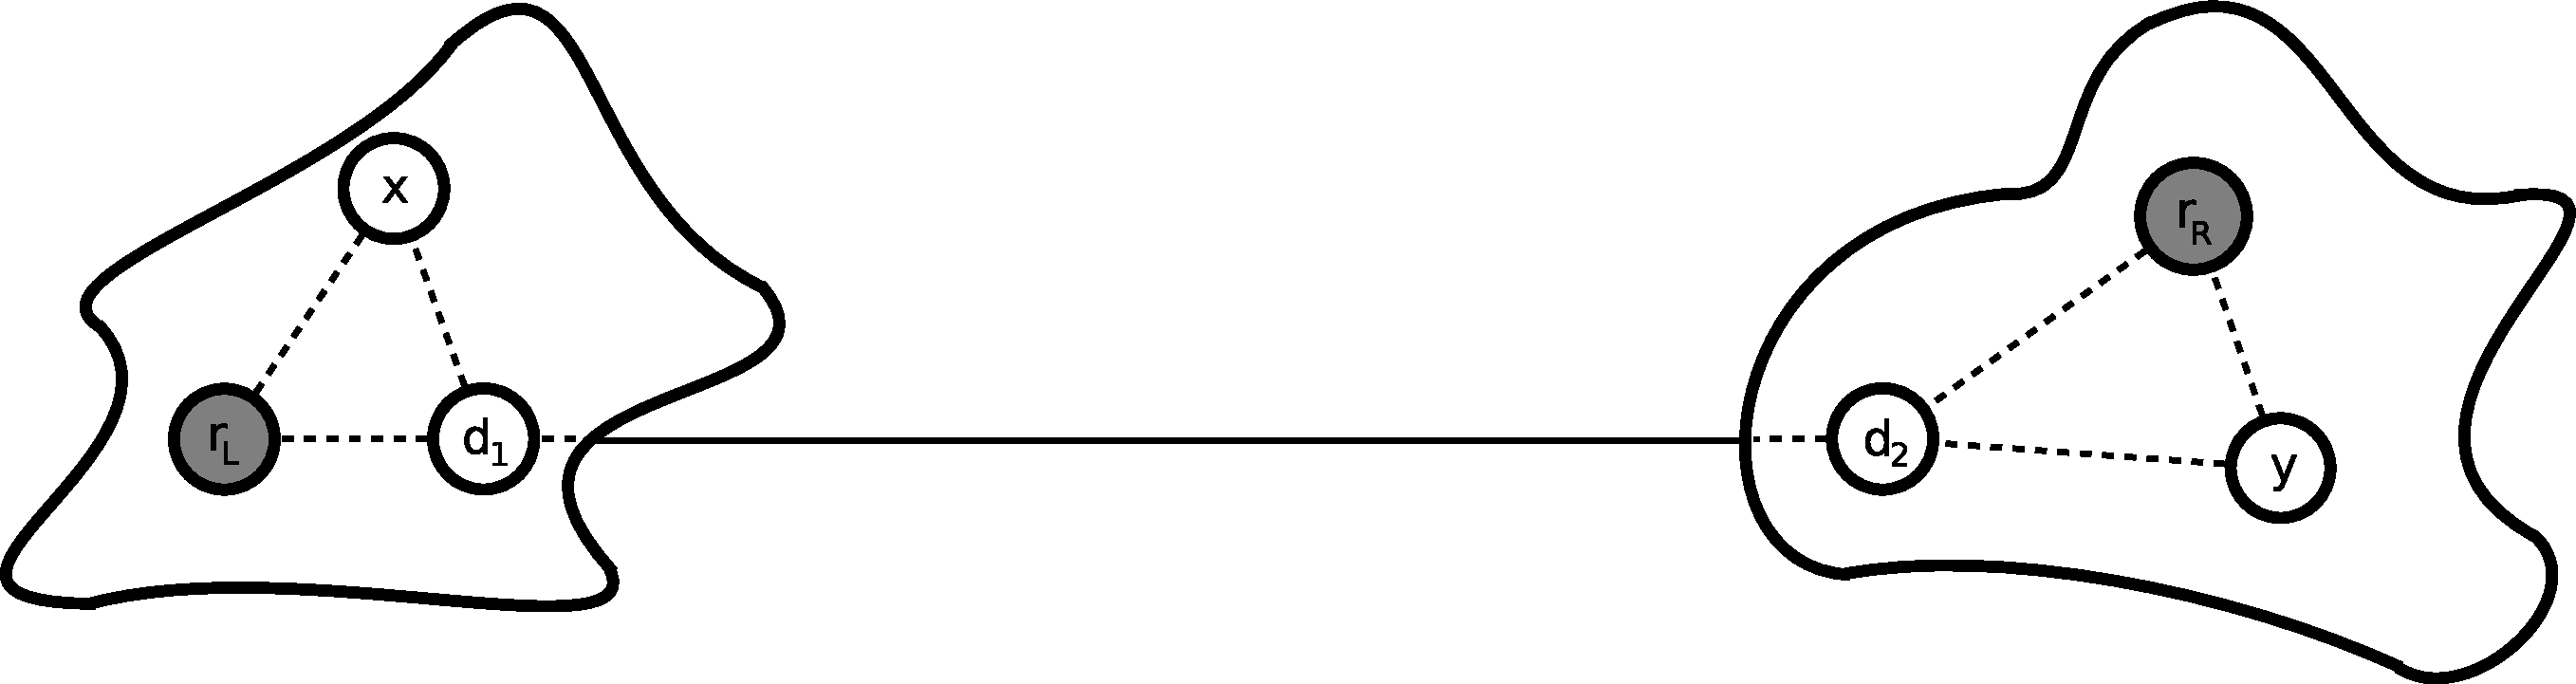
\includegraphics[width=420pt]{bilder/bew5.pdf}
	\caption{Ein Graph mit zwei über eine Kante verbundenen Teilgraphen mit jeweils einem Element aus der metrischen Basis}
  	 \end{figure}
  Angenommen es existiert ein nicht getrenntes Knotenpaar $x,y$. Sei $d_1$ der Bifurkator von $y,x,r_L$ und $d_2$ der Bifurkator von $x,y,r_R$. Dann gilt: $$dist(r_L,x) \leq dist(r_L,d_1)+ dist(d_1,x)$$ $$dist(r_R,y) \leq dist(r_R,d_2)+ dist(d_2,y)$$ $$dist(r_L,y) > dist(r_L,d_1)+ dist(d_2,y)$$ $$dist(r_R,x) > dist(r_R,d_2)+ dist(d_1,x)$$
  Da $x$ und $y$ nicht getrennt sind, gilt:
   $$dist(r_R,y) =dist(r_R,x),\: dist(r_L,x) = dist(r_L,y)$$ Dies kann eingesetzt und umgeformt werden zu dem folgenden Widerspruch:
  $$\Rightarrow dist(r_L,d_1)+ dist(d_1,x) \geq dist(r_L,x) = dist(r_L,y)> dist(r_L,d_1)+ dist(d_2,y)$$
  $$\Leftrightarrow dist(r_L,d_1)+ dist(d_1,x) > dist(r_L,d_1)+ dist(d_2,y)$$
  $$\Leftrightarrow dist(d_1,x) >  dist(d_2,y)$$
  
  $$\Rightarrow dist(r_R,y) \leq dist(r_R,d_2)+ dist(d_2,y) < dist(r_R,d_2) + dist(d_1,x) < dist(r_R,x)$$
  $$\Leftrightarrow dist(r_R,y) < dist(r_R,x) = dist(r_R,y)$$
  $$\Leftrightarrow dist(r_R,y) < dist(r_R,y) \lightning $$  
  
\end{proof}
\begin{lem}
\label{lem2}
\label{sepvertex}
Die Kontraktion von Trennungsknoten vom Grad zwei oder die Knotenerweiterung hat keinen Einfluß auf die metrische Dimension eines Graphens.
\end{lem}
\begin{proof}[Beweis:]
Sei ein Graph $G$ mit einer metrischen Basis $R_k$ und einem Trennungsknoten $v_s$ mit $deg(v_s)=2$ gegeben. Die zwei Teilgraphen welche durch das Entfernen von $v_s$ entstehen bezeichne man als $G_R$ und $G_L$.\\Der Graph $G'$ resultiert durch die Kontraktion von $v_s$ mit einem beliebigen Nachbarn.
\begin{floatingfigure}[l]{200pt}
\centering
\includegraphics*[width = 200pt]{bilder/proof4,2.pdf}
\caption{Ein Graph mit einem Trennungknoten vom Grad zwei}
\end{floatingfigure}
\vspace{-2mm}
Angenommen die metrische Dimension in $G'$ ist größer als in $G$, dann existiert ein\\Knotenpaar $x,y$, welcher in $G$ getrennt wird, aber nicht in $G'$.\\Also gibt es mindestens einen Knoten in der metrischen Basis $R_K$ von dem Graphen $G$, welcher $x,y$ trennt.\\Sei dies der Knoten $r_k$. Dieser Knoten trennt  $x,y$ nicht in dem Graphen $G'$.\\
Betrachte nun die Fälle einzeln: Falls alle drei Knoten in dem gleichen Teilgraphen sind,\\so ist $v_s$ in keinem kürzesten Weg enthalten und $x,y$ bleiben getrennt, sofern sie zuvor getrennt waren. Sind die Knoten $x,y$ in einem Teilgraphen und $r_k$ in dem Anderen, so schrumpft die kürzeste Wege Distanz von $r_k$ zu $x$ und zu $y$ um genau eins und bleibt dabei unterschiedlich auch in $G'$. Betrachte nun den Fall dass die Knoten $x$ und $y$ in unterschiedlichen Teilgraphen sind:
\begin{enumerate}
\item[1. Fall] Angenommen jeder der Teilgraphen $G_R$ und $G_L$ beinhalten mind. ein Element aus der metrischen Basis. Der Widerspruch folgt unmittelbar aus dem Satz \ref{first_theorem}.
\item[2. Fall] Angenommen einer der Tielgraphen beinhaltet kein Element der metrischen Basis, sei dies o.B.d.A $G_R$.
Dadurch das dieser Teilgraph kein Element der metrischen Basis beinhaltet und genau einen Trennungsknoten besitzt folgt aus dem Satz \ref{sepvertex} das die metrische Dimension von $G_R$ höchstens eins ist und da $G_R$ nicht leer ist gilt nach Satz \ref{path} dass $G_R$ ein Weg ist. Falls ein nichtgetrenntes Paar von Knoten $x,y$ existiert mit o.B.d.A. $x$ ist im Teilgraphen $G_R$, dann war in $G$ das Knotenpaar $x$ und der Vorgänger von $y$ nicht getrennt. Damit ist auch der letzte Widerspruch gezeigt.
\end{enumerate}
\end{proof}
%%%%%%%%%%%%%%%%%%%%%%%%%%%%%%%%%%%%%%%%%%%%%%%%%%%%%%%%%%%%%%%%%%%%%%%%%%%%%%%%%%%%%%%%%%%%%%%%%%%%%%%%%%%%%%%%
\subsection{Metrische Dimension vom Freundschaftsgraphen $F_{n}$}
''Haben je zwei Bekannte einen weiteren gemeinsamen Bekannten, so gibt es eine Person, welche alle Anderen kennt''. Diese Behauptung kann durch als ein Graphenproblem definiert werden, wobei Knoten Personen und Kanten Bekannschaften repräsentieren.  Dieser von Paul Erdős etc. in \cite{Erdos} eingeführte Graph wird als Freundschaftsgraph bezeichnet. In dem Paper von Imran etc. wird die Partitionsdimension der Freundschaftsgraphen bestimmt und in diesem Kapitel seine metrische Dimension.
\begin{defi}{\textbf{(Freundschaftsgraph $F_n$)}}\\
\emph{Seien $n$ Kreise $C_3$ mit der Knotenfolge $|V|=\{v_1,v_2,v_3\}$ gegeben. Durch das Verschmelzen von allen Knoten, welche mit $v_1$ gekenntzeichnet sind entsteht der Freundschaftsgraph $F_n$. Dieser Graph hat die Ordnung $2n+1$ und die Größe $3n$.}
\end{defi}
\begin{bsp}\textcolor{white}{lala}
\begin{figure}[h!]
\centering
 		 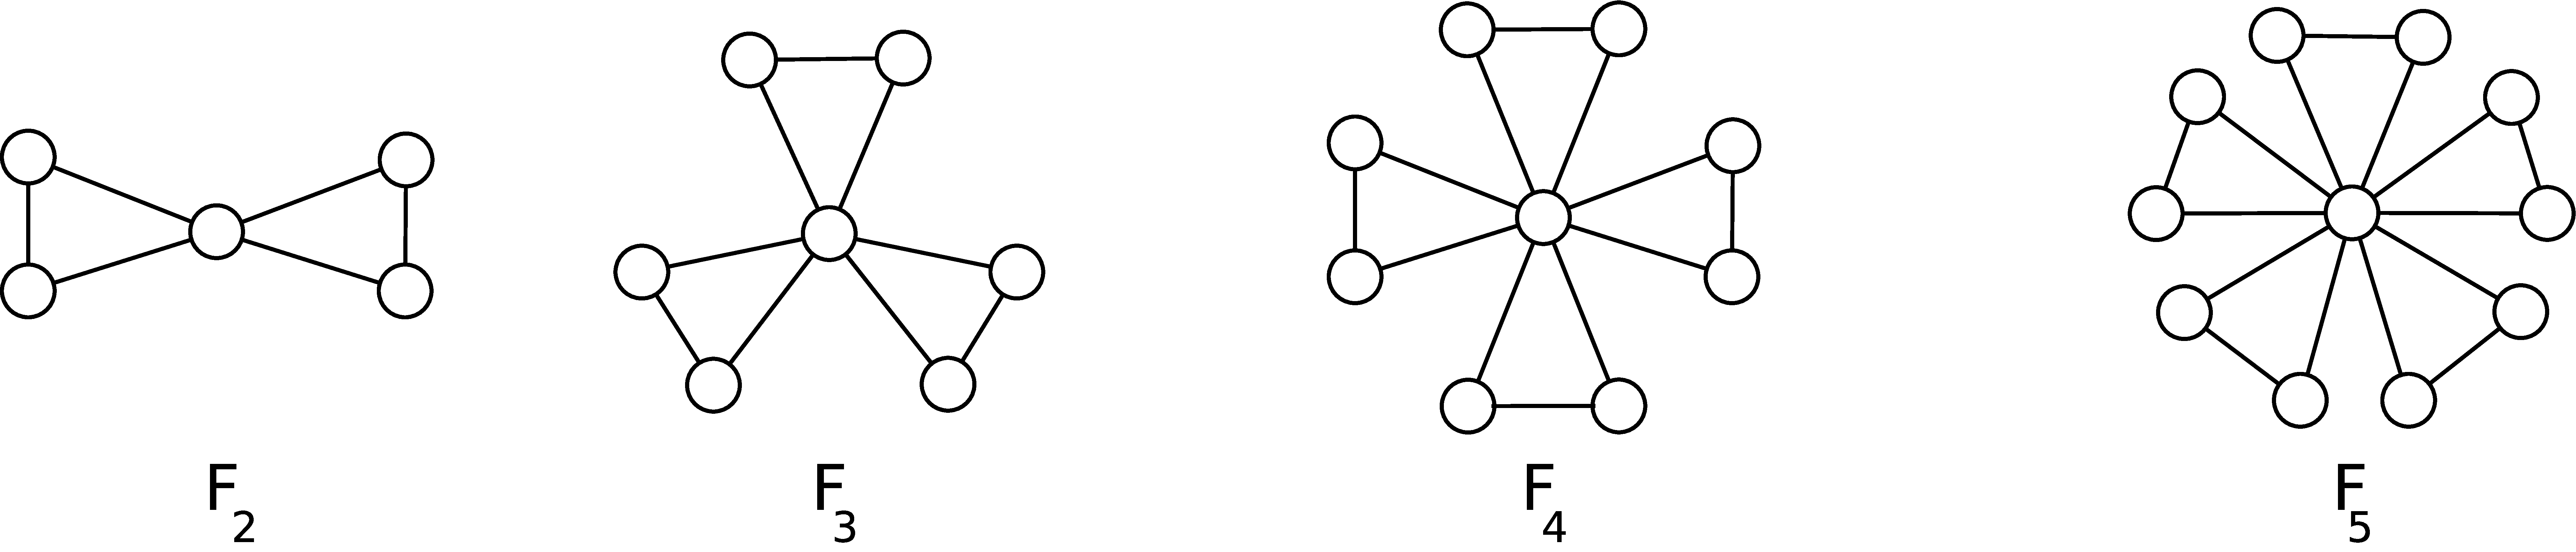
\includegraphics[width=428pt]{bilder/freunschaftsgraph.pdf}
   \caption{Vier Freundschaftsgraphen}
   \label{bild:fg}
\end{figure}
\end{bsp}
\begin{lem}
\label{Freundschaftsgraphen}
Die metrische Dimension eines Freundschaftsgraphen $F_n$ ist $n$.
\end{lem}
\vspace{-1mm}
Um diese Behauptung zu beweisen, wird das folgende Lemma benötigt. 
\begin{lem}
\label{mindfreundschaftsgraph}
Sei ein Freundschaftsgraph $F_n$ gegeben. Jede metrische Basis muss aus jedem $C_3$ mindestens einen der folgenden Knoten $\{v_{2},v_{3}\}$ beinhalten.
\end{lem}
\newpage
\begin{proof}[Beweis:]
\textcolor{white}{lala}
\begin{floatingfigure}[l]{200pt}
\centering
\includegraphics*[width = 100pt]{bilder/freundschaftsgraphbew.pdf}
\caption{Ein markierter $C_{3}$}
\end{floatingfigure}
Angenommen keiner dieser Knoten ist\\in der metrischen Basis. Durch die eindeutige Verbindung zu dem Restgraphen, welche über einen Trennungsknoten läuft, folgt aus\\Symmetriegründen dass die Knoten $v_{2}$ und $v_{3}$ identische Markierungen haben.\\Dies ist ein Widerspruch zu der Definition einer metrischen Basis.\\
Damit ist die metrische Dimension eines\\Freundschaftsgraphen $F_n$ mindestens gleich der Anzahl seiner $C_{3}$ und damit mindestens $n$.\textcolor{white}{lala}\\\textcolor{white}{lala}
\end{proof}
\vspace{-6mm}
\begin{proof}[Beweis von Lemma \ref{Freundschaftsgraphen}:]
\textcolor{white}{lala}\\
Nach Lemma \ref{mindfreundschaftsgraph} ist bekannt, dass die metrische Dimension eines Freundschaftsgraphen $F_n$ mindestens $n$ ist. Angenommen alle als $v_2$ markierten Knoten werden in die metrische Basis aufgenommen, damit sind sie getrennt. Der Knoten $v_1$ hat die Distanz eins zu allen Knoten in der metrischen Basis und ist der einzige Knoten mit dieser Eigenschaft. Für jeden Knoten $v_3$ gibt es genau einen Knoten $v_2$ mit der Distanz eins und zu allen anderen Knoten in der metrischen Basis hat er die Distanz zwei. Alle Markierungen sind eindeutig und der gesammte Graph ist durch die $n$ Knoten getrennt.
\end{proof}

%%%%%%%%%%%%%%%%%%%%%%%%%%%%%%%%%%%%%%%%%%%%%%%%%%%%%%%%%%%%%%%%%%%%%%%%%%%%%%%%%%%%%%%%%%%%%%%%%%%%%%%%%%%%%%%%
\subsection{Metrische Dimension von Sonnengraphen $S_{n,k}$}
\begin{defi}{\textbf{(Sonnengraph $S_{n,k}$)}}\\
\emph{Sei ein Kreis $C_n$ für $n \geq 3$ mit der Knotenmenge $|V|=\{ c_1, \ldots , c_n \}$ und $n$ Weggraphen $P_{k-1}$ für $k\geq 2$ gegeben. Die Knoten mit Grad eins auf dem $i$-ten Weg werden als $v_{i,1}$ und $v_{i,k-1}$ bezeichnet. Durch das Hinzufügen von $n$ neuen Kanten der Form $\{v_{i,1},c_i\}$ für $1 \leq i \leq n$ ensteht der zusammenhängende Sonnengraph $S_{n,k}$.\\
Alle als $v_{i,k-1}$ bezeichneten Knoten werden Endknoten genannt, als $c_i$ bezeichneten Knoten werden Ursprungsknoten genannt und eine Knotenmenge mit den Knoten $\{c_i,v_{i,1}, \ldots ,v_{i,k-1}\}$ für $1 \leq i \leq n$ als Strahl.\\
Für $n=1$ ist der Graph der Sterngraph aus Definition \ref{defstern}.}
\end{defi}
\begin{bsp}\textcolor{white}{lala}
\begin{figure}[h!]
\centering
 		 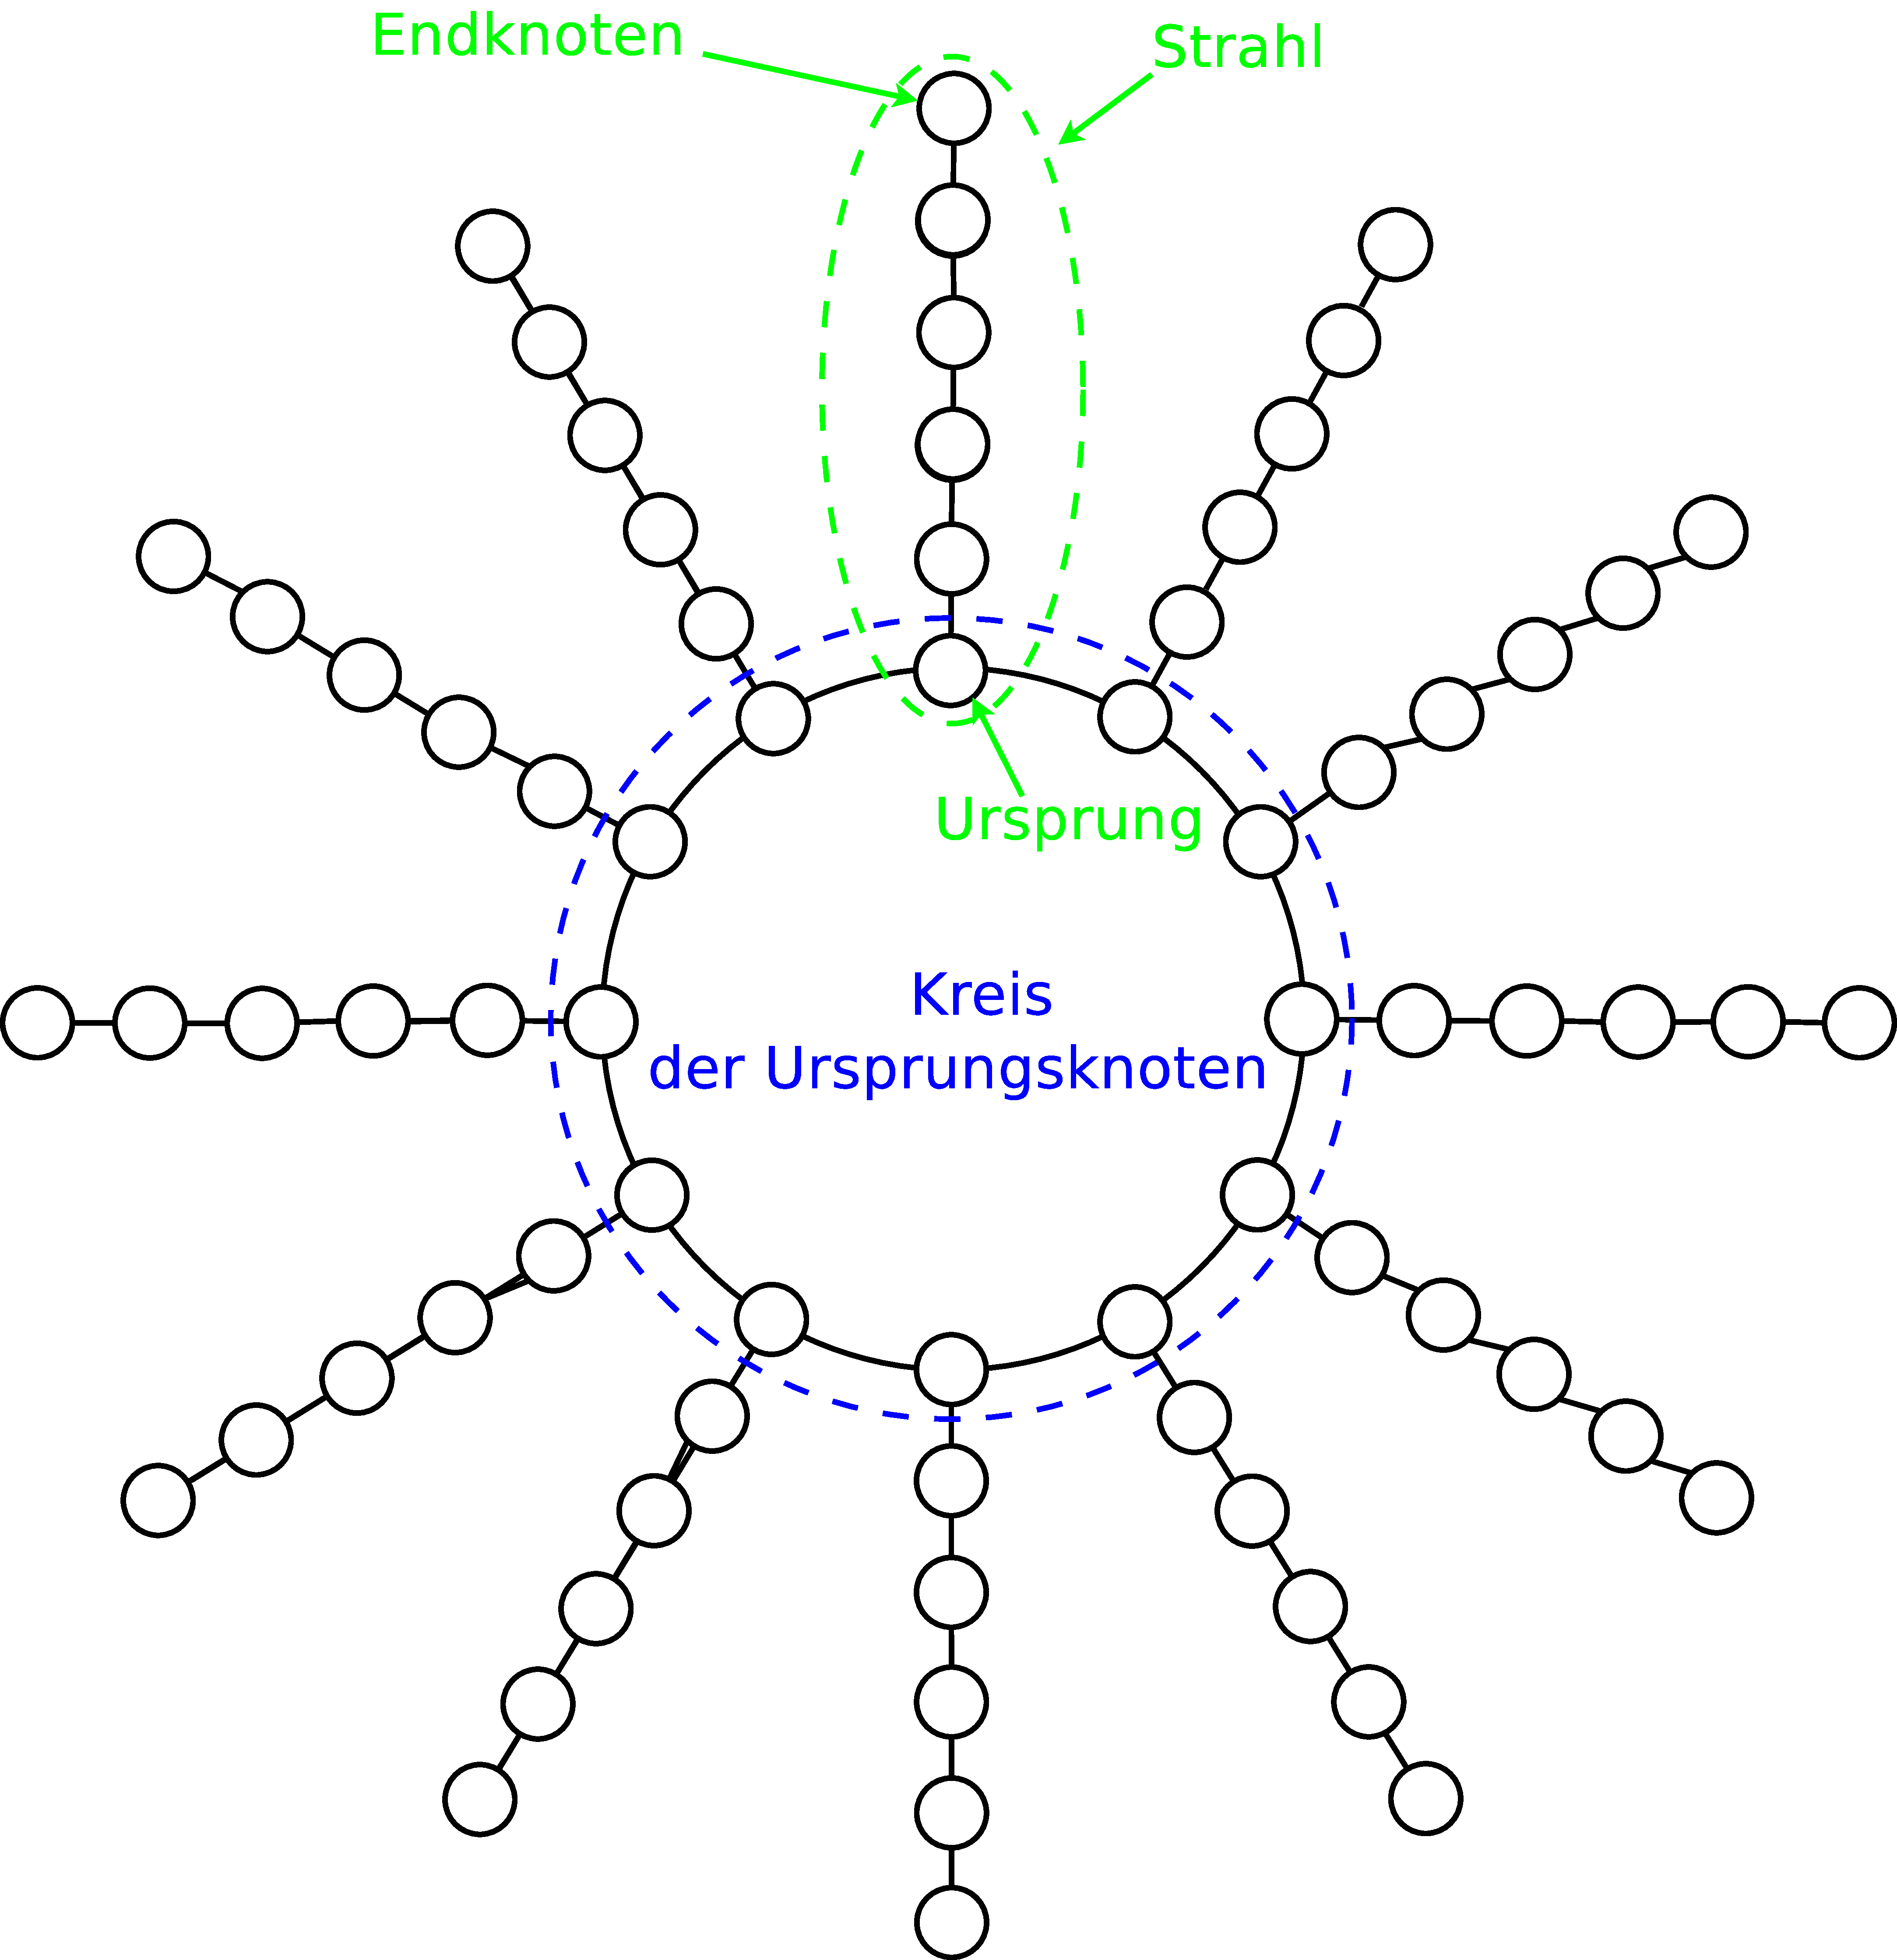
\includegraphics[width=200pt]{bilder/sonne.pdf}
   \caption{Der Sonnengraph $S_{12,6}$}
   \label{bild:sonnengraph}
\end{figure}
\end{bsp}
\begin{lem}
Die metrische Dimension (MD) eines Sonnengraphen $S_{n,k}$ mit $n \geq 3$ und $k \geq 1$ ist zwei. 
\end{lem}
\begin{proof}[Beweis:]
\begin{figure}[h!]
		\centering
 		 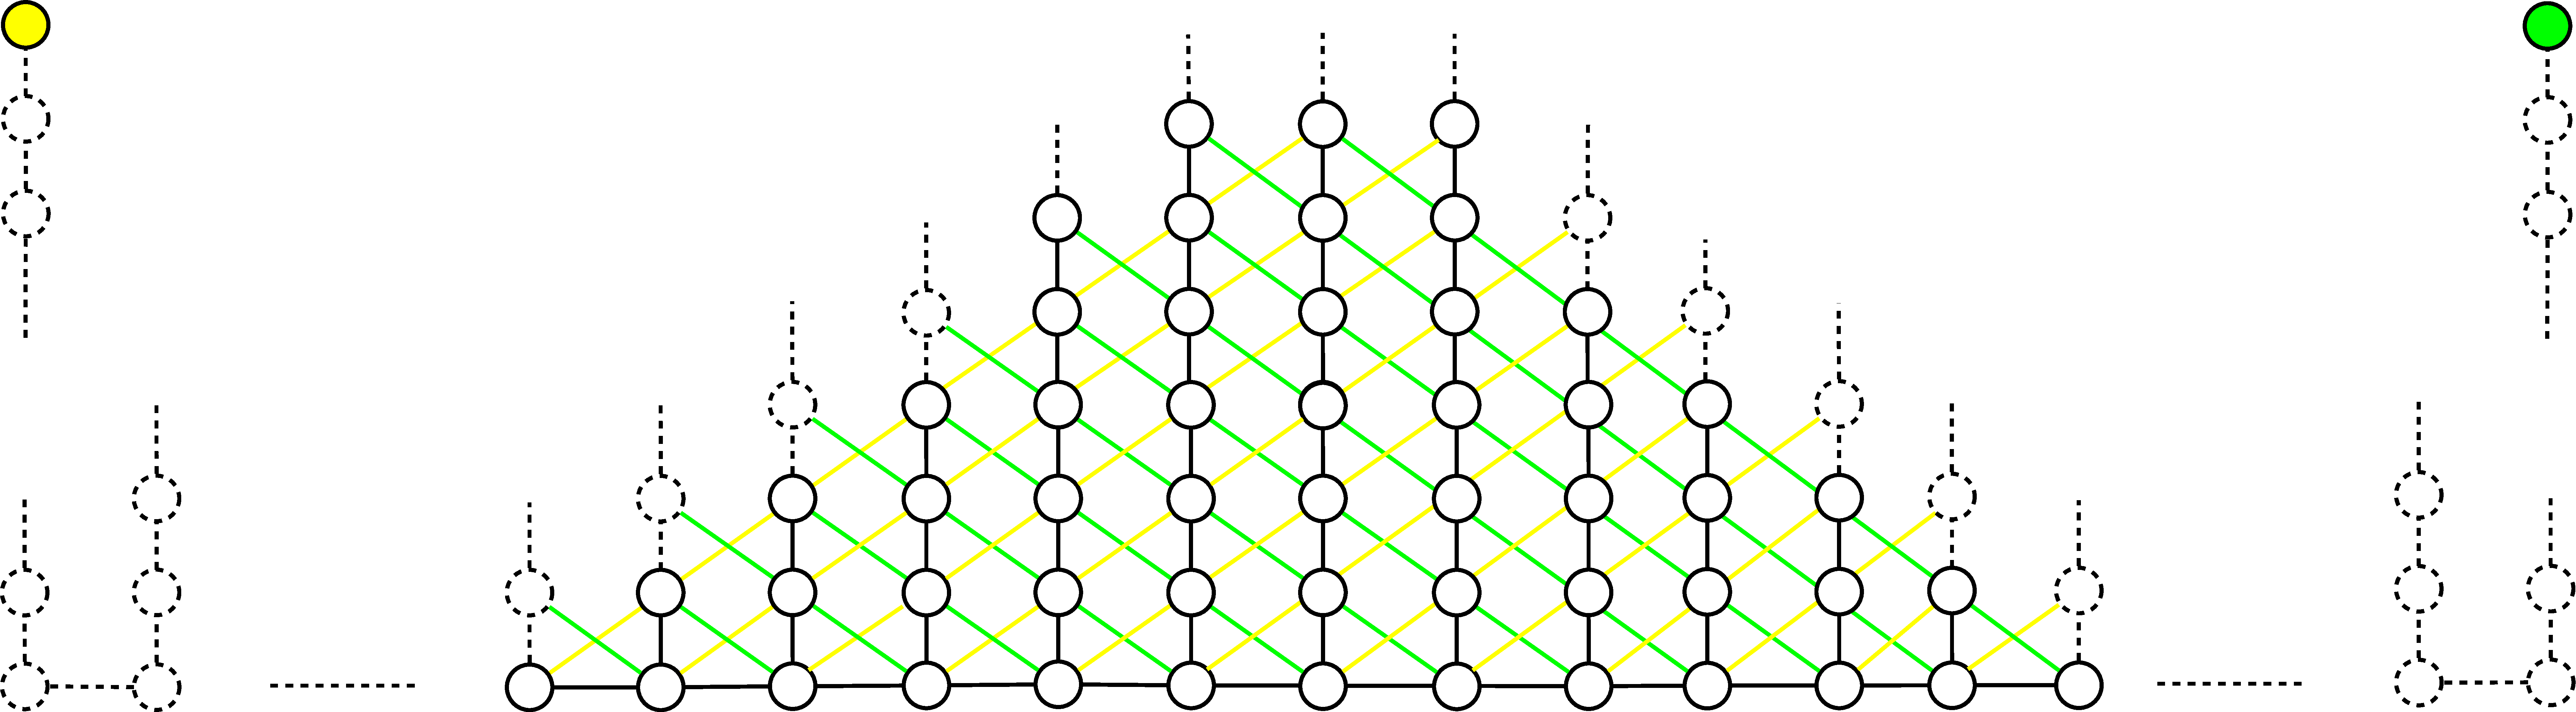
\includegraphics[width=430pt]{bilder/sonne1.pdf}
   \caption{Ein $C_{n}$-$Blatt$ wird durch zwei Knoten getrennt}
  	 \end{figure}
  	 
  	 \begin{figure}[h!]
		\centering
 		 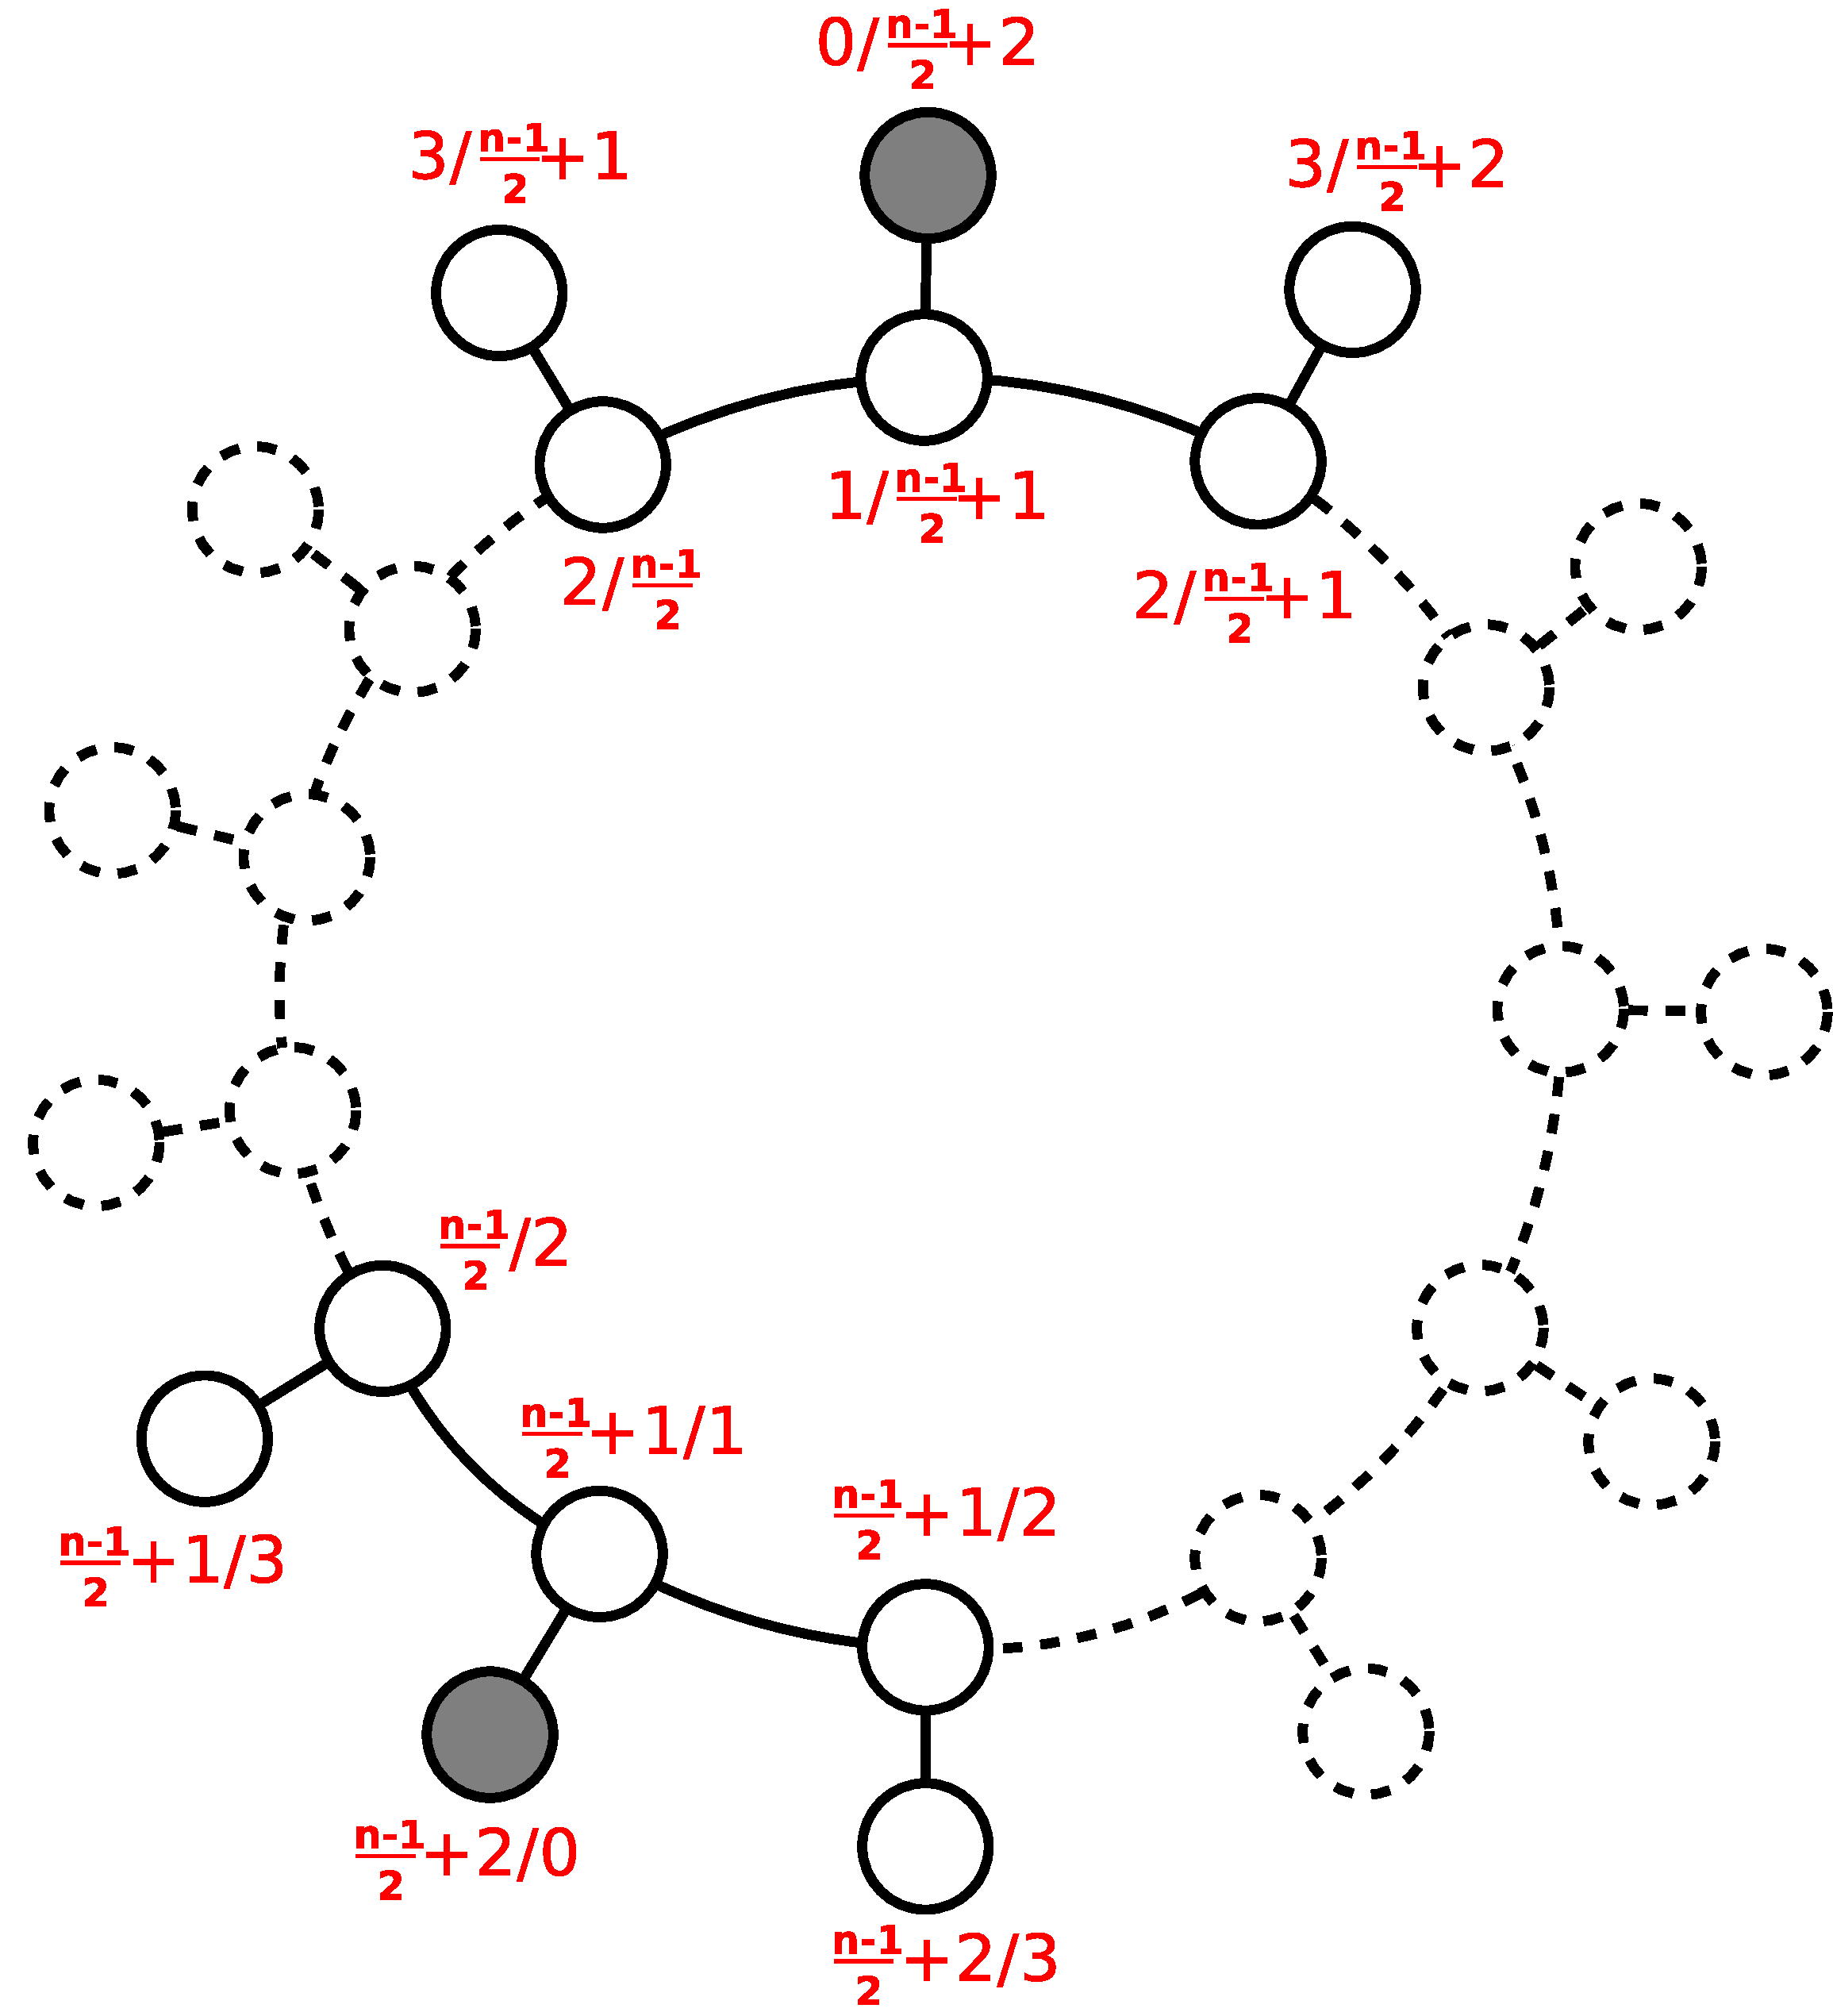
\includegraphics[width=300pt]{bilder/sonne2.pdf}
   \caption{Der Sonnengraph $S^*_{2n,k}$}
  	 \end{figure}
  	 Jeder Knoten auf einem Strahl hat eine $a+x/b+x$ Markierung mit $0 \leq x \leq k$ und $a/b$ die Markierung vom Strahlursprung auf dem Kreis $C_n$.
\end{proof}  	 
\clearpage
%%%%%%%%%%%%%%%%%%%%%%%%%%%%%%%%%%%%%%%%%%%%%%%%%%%%%%%%%%%%%%%%%%%%%%%%%%%%%%%%%%%%%%%%%%%%%%%%%%%%%%%%%%%%%%%%
\subsection{Metrische Dimension von $C_j$-Bäumen}
In diesem Kapitel wird eine neue Graphklasse eingeführt. Es sind Bäume mit der Eigenschaft, dass Knoten mit größerem Grad als zwei durch Kreise ersetzt werden. Das Kapitel widmet sich der Bestimmung der metrischen Dimension solcher Graphen sowie dem Vergleich der metrischen Dimension von den ursprünglichen Bäumen gegenüber den mit den Kreisen erweiterten. Zunächst fangen wir mit einem Spezialfall von solchen Graphen, den $C_3$-$Bäumen$, an.
\subsubsection{Metrische Dimension von $C_3$-Bäumen}
\begin{defi}
\label{C_{3} tree}
Für einen gegebenen Baum $T=(V,E)$ mit $deg(v_i)\leq 3$ für $v_i \in V$. Sei $$V'=\{v_k|v_k \in V \wedge deg(v_k)=3\}\subseteq V$$ eine Teilmenge der Knoten von dem Graphen $T$. Ersetze jedes Element $v_j \in V'$ durch einen $C_3$ (diese Teilgraphen werden als \emph{$C_{3,j}$} bezeichnet), so dass jeder Knoten vom $C_{3,j}$ mit genau einem Nachbarn von $v_j$ verbunden wird. Die drei Nachbarn vom $C_{3,j}$ werden als \emph{$C_{3,j}$-$Kinder$} bezeichnet. Sofern zwei von den $C_{3,j}$-$Kinder$ Blätter sind, so bezeichnet man den Teilgraphen mit dem $C_{3,j}$ und seinen Nachbarn als \emph{$C_{3}$-$Blatt$}. Da der entstandene Graph nur Kreise der Länge drei beinhaltet, wird er als \emph{$C_3$-$Baum$} bezeichnet. 
   \end{defi}
Die $C_3$-$Bäume$ bestehen nur aus Knoten vom Grad eins, zwei und drei, außerdem haben die einzigen Kreise, die diese Graphen beinhalten, die Länge drei. Dies bedeutet insbesondere, dass alle Knotenpaare, die nicht Teil des gleichen $C_3,j$ sind, einen eindeutigen Weg haben. Das macht jeden Knoten vom Grad zwei zu einem Trennungsknoten. Damit können diese Knoten für die Berechnung der metrischen Dimension in dem Graphen kontrahiert werden nach Satz \ref{sepvertex}.
\begin{bsp} \textcolor{white}{lala} \vspace{-6mm}
\begin{figure}[h!]
		\centering 		 
   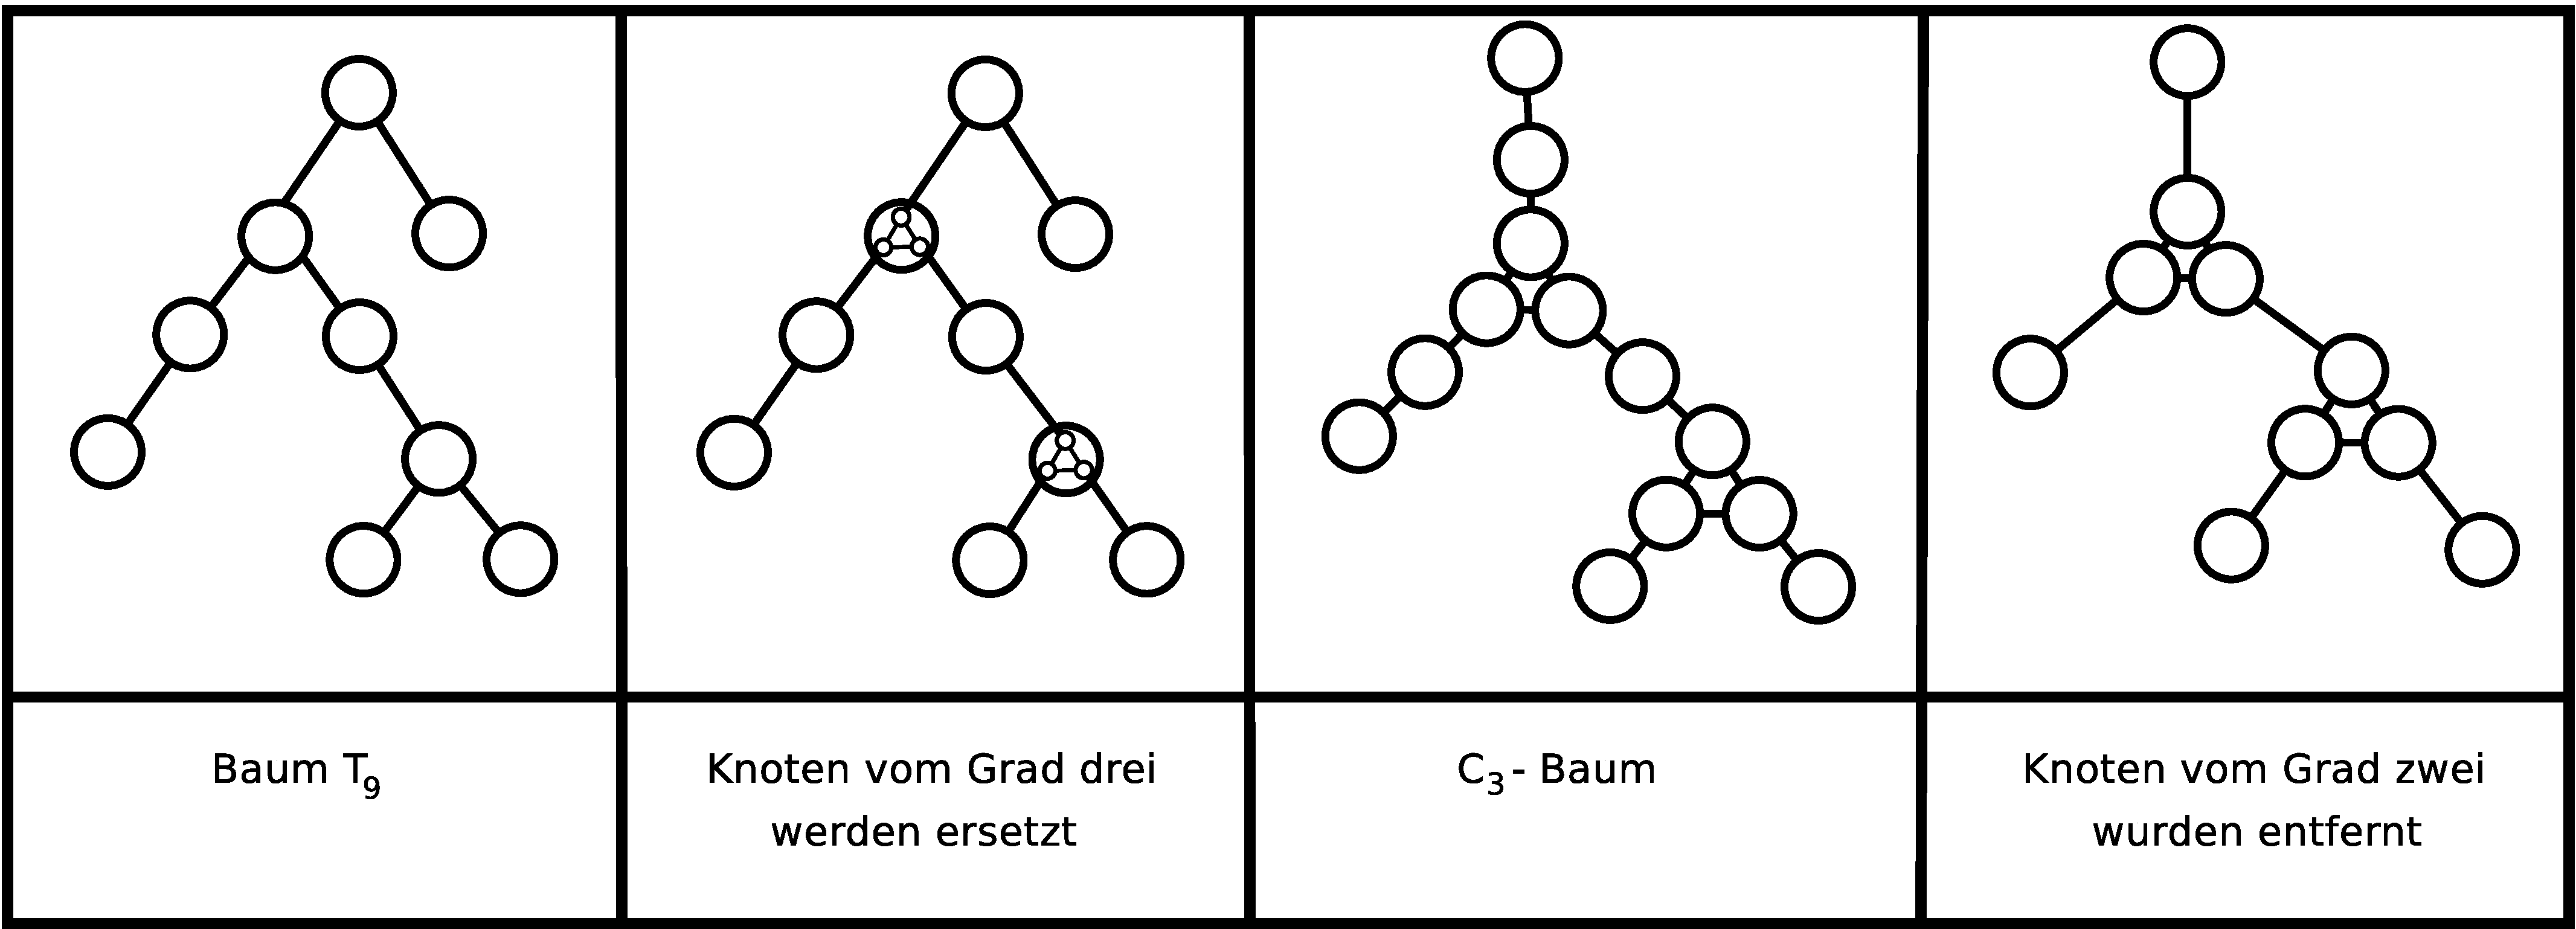
\includegraphics[width=420pt]{bilder/trees.pdf}
	\caption{Entwicklung von einem Baum zum $C_{3}$-$Baum$ und anschließender Knotenkontraktion}
  	 \end{figure}
\end{bsp}
Gegeben sei der abgebildete Baum $T_9$ mit neun Knoten. Dieser Baum enthält zwei Knoten von Grad drei, welche jeweils wie in der Definition beschrieben durch einen $C_3$ ersetzt werden. Um die Berechnung der metrischen Dimension des enstandenen Graphen zu erleichtern, werden alle Knoten vom Grad zwei kontrahiert.
Die metrische Dimension eines Graphen $G$ mit mindestens zwei $C_{3,j}$ ist gleich der Anzahl von seiner $C_{3}$-$Blätter$.
\begin{lem}
Sei $C_{3,j}$ ein beliebiges $C_{3}$-$Blatt$. Jede metrische Basis muss mindestens eine der folgenden Knoten $\{v_{j,1},v_{j,2},v_{j,3},v_{j,4}\}$ beinhalten.
\end{lem}
\begin{proof}[Beweis:]
\textcolor{white}{lala}
\begin{floatingfigure}[l]{200pt}
\centering
\includegraphics*[width = 100pt]{bilder/beweis.pdf}
\caption{Ein markiertes $C_{3}$-$Blatt$}
\end{floatingfigure}
Angenommen keiner dieser Knoten ist\\in der metrischen Basis. Durch die eindeutige Verbindung zu dem Restgraphen, welche über einen Trennungsknoten läuft, folgt aus\\Symmetriegründen dass die Knoten $v_{j,3}$ und $v_{j,4}$, sowie $v_{j,1}$ und $v_{j,2}$ identische Markierungen haben.\\Dies ist ein Widerspruch zu der Definition einer metrischen Basis.\\
Damit ist die metrische Dimension eines Graphens $G$ mit mindestens zwei $C_{3,j}$\\mindestens gleich der Anzahl von seinen $C_{3}$-$Blätter$.\textcolor{white}{lala}\\\textcolor{white}{lala}
\end{proof}
\textcolor{white}{lala} \vspace{-6mm}
\begin{lem}
Die metrische Dimension (MD) eines Graphen $G$ mit mindestens zwei $C_{3,j}$ ist nicht größer als die Anzahl seiner $C_{3}$-$Blätter$. 
\end{lem}
\textcolor{white}{lala} \vspace{-6mm}
%Um diese Eigenschaft zu beweisen werden zwei Sätze über die Struktur solcher $C_{3}$-$Bäume$ benötigt.
\begin{lem}
\label{bkb}
Jeder Knoten eines $C_{3}$-$Baumes$, welcher kein Blatt ist, ist ein Trennungsknoten.
\end{lem}


\begin{proof}[Beweis:]
Angenommen es gibt einen Knoten $u$, welcher kein Blatt ist und kein Trenunngsknoten. Da der Graph nur aus Knoten von Grad drei und Grad eins besteht ist der Knotengrad von $u$ drei. Dies bedeutet $u$ hat genau drei Nachbaren $v,w,x$. Da
der Knoten $u$ nach Annahme kein Trennungsknoten ist, gibt es einen Weg zwischen jedem Paar seiner Nachbarknoten.
\begin{itemize}
\item Fall I: Ein Nachbarknoten ist ein Blatt.\\ Es kommt direkt zum Widerspruch, da durch das Löschen von $u$ sich der Knotengrad von dem Blatt um eins verkleinert und damit null wird, also ein getrennter einzelner Knoten ist.
\item Fall II: Alle Nachbarknoten haben den Grad drei.\\
Es muss immernoch einen Weg zwischen jedem Knotenpaar geben damit der Graph zusammenhängend ist. Somit gibt es auch einen Weg über alle drei Knoten, sei der Anfangsknoten von diesem Weg o.B.d.A. der Knoten $v$, der Endknoten o.B.d.A. der Knoten $x$ und die Länge dieses Weges ist zwangsläufig mindestens drei. Wird wieder der entfernte Knoten $u$ betrachtet so folgt, dass der Graph einen Kreis beinhaltet welcher aus dem Weg von $v$ zu $x$ besteht und über den entfernten Knoten $u$ zurück zum Knoten $v$ geht.\\
Damit gibt es in dem Graphen mind. einen Kreis mit einer echt größeren Länge als drei und dies ist ein Widerspruch zur Definition des $C_{3}$-$Baumes$, welche nur Kreise der Länge drei erlaubt.
\end{itemize}
\end{proof}
\begin{lem}
\label{bkb2}
In jedem Teilgraphen eines $C_{3}$-$Baumes$ mit mindestens vier Knoten ist mindestens ein Knoten aus der metrischen Basis.
\end{lem}
\begin{proof}[Beweis:]
Der kleinste Teilgraph der durch das Löschen eines Knotens entstehen kann ist ein Blatt. Dieser besteht allerdings nur aus einem Knoten. Der nächstgrößere Teilgraph der durch das Löschen eines Knotens entstehen kann beinhaltet vier Knoten,genauer den unteren Teil eines $C_{3}$-$Blattes$. Damit beinhaltet er auch sein linkes Blatt, welches in die metrische Basis aufgenommen wird. Jeder größere Teilgraph beinhaltet diese vier Knoten. %Unabhängig davon welcher Knoten als Wurzel verwendet wurde, galt bei dem ursprünglichen Baum dass der Knoten mit der weitesten Entfernung von der Wurzel(der Knoten davor), hatte genau zwei Kinder und aus dem wurde ein $C_{3,j}$-$Blatt$.  
\end{proof}
\begin{proof}[Beweis von Lemma 27:]
Der gesamte Graph besteht nur aus Knoten vom Grad drei oder Grad eins. In die metrische Basis wird das linke Blatt von jedem $C_{3}$-$Blatt$ aufgenommen. Sei $n$ die Anzahl der $C_{3}$-$Blätter$ und $m$ die Anzahl der $C_{3,j}$, die keine $C_{3}$-$Blätter$ sind und bei diesem Beweis als einfache $C_{3,j}$ bezeichnet werden.\\
\begin{itemize}
\item Fall I. Die Knoten $u$ und $v$ haben unterschiedliche Distanzen vom Knoten $r_1$ aus der metrischen Basis. Der Knoten $r_1$ trennt die Knoten $u$ und $v$.
\item Fall II. Die Knoten $u$ und $v$ haben die gleiche Distanz vom Knoten $r_1$ aus der metrischen Basis und die Knoten $u$ und $v$ liegen im selben $C_{3,j}$.\\
O.B.d.A. sei $b_1$ der ausgewählte Knoten $r_1$ oder $b_1$ auf allen kürzesten Wegen von dem Knoten $r_1$ zu jedem Knoten in dem $C_{3,j}$. Es gibt zwei nicht getrennte Knotenpaare durch den Knoten $r_1$, das Knotenpaar $\{b_2,b_3\}$ oder das Knotenpaar $\{c_2,c_3\}$.\\
Angenommen $b_2$ und $b_3$ sind Blätter (daraus folgt das $b_1$ kein Blatt sein kann), so wird o.B.d.A. $b_3$ in die metrische Basis aufgenommen und so ist seine Markierung o.B.d.A. an der ersten Position $0$ und er ist der einzige Knoten mit dieser Markierung. Sein einziger Nachbar $c_3$, bekommt die Markierung $1$ an der ersten Position, damit ist dieser Knoten auch eindeutig markiert. Die anderen zwei Knoten $c_1$ und $c_2$ auf dem $C_3$ bekommen die Markierung $2$ an der ersten Position und ihre zwei Nachbaren $b_1$ und $b_2$, die Markierung $3$ an der ersten Position. Somit kriegen die Knotenpaare $b_2$ und $b_3$ und $c_2$ und $c_3$ unterschiedliche Markierungen und sind getrennt.\\ 	 
Sei nun $b_3$ kein Blatt, damit ist er Teil eines anderen $C_{3,j}$, welcher zwei $C_{3,j}$-$Kinder$ besitzt. Sind beide $C_{3,j}$-$Kinder$ keine Blätter, so sind sie Teile eines anderen $C_{3,j}$. Damit ist $b_3$ nach Satz \ref{bkb} ein Trennungsknoten. Der Graph ohne die Knoten $b_1$ und $b_2$ beinhaltet mindestens vier Knoten, die anderen Knoten auf diesem $C_{3,j}$ und ihre zwei $C_{3,j}$-$Kinder$ und nach Satz \ref{bkb2} mindestens ein Element aus der metrischen Basis.\\
Da der Knoten $b_3$ ein Trennungsknoten ist, ist die Distanz von diesem Knoten zu $b_3$ ist echt kleiner als zu jedem anderen Knoten in dem ausgewählten $C_{3,j}$. Die Markierung von $b_3$ sei o.B.d.A. an der ersten Position $a$. Sein einziger Nachbar $c_3$, bekommt die Markierung $a+1$ an der ersten Position. Die anderen zwei Knoten $c_1$ und $c_2$ auf dem $C_3$ bekommen die Markierung $a+2$ an der ersten Position und ihre zwei Nachbaren $b_1$ und $b_2$, die Markierung $a+3$ an der ersten Position. Somit kriegen die Knotenpaare $b_2$ und $b_3$ und $c_2$ und $c_3$ unterschiedliche Markierungen und sind getrennt.
\begin{figure}[h!]
		\centering
 		 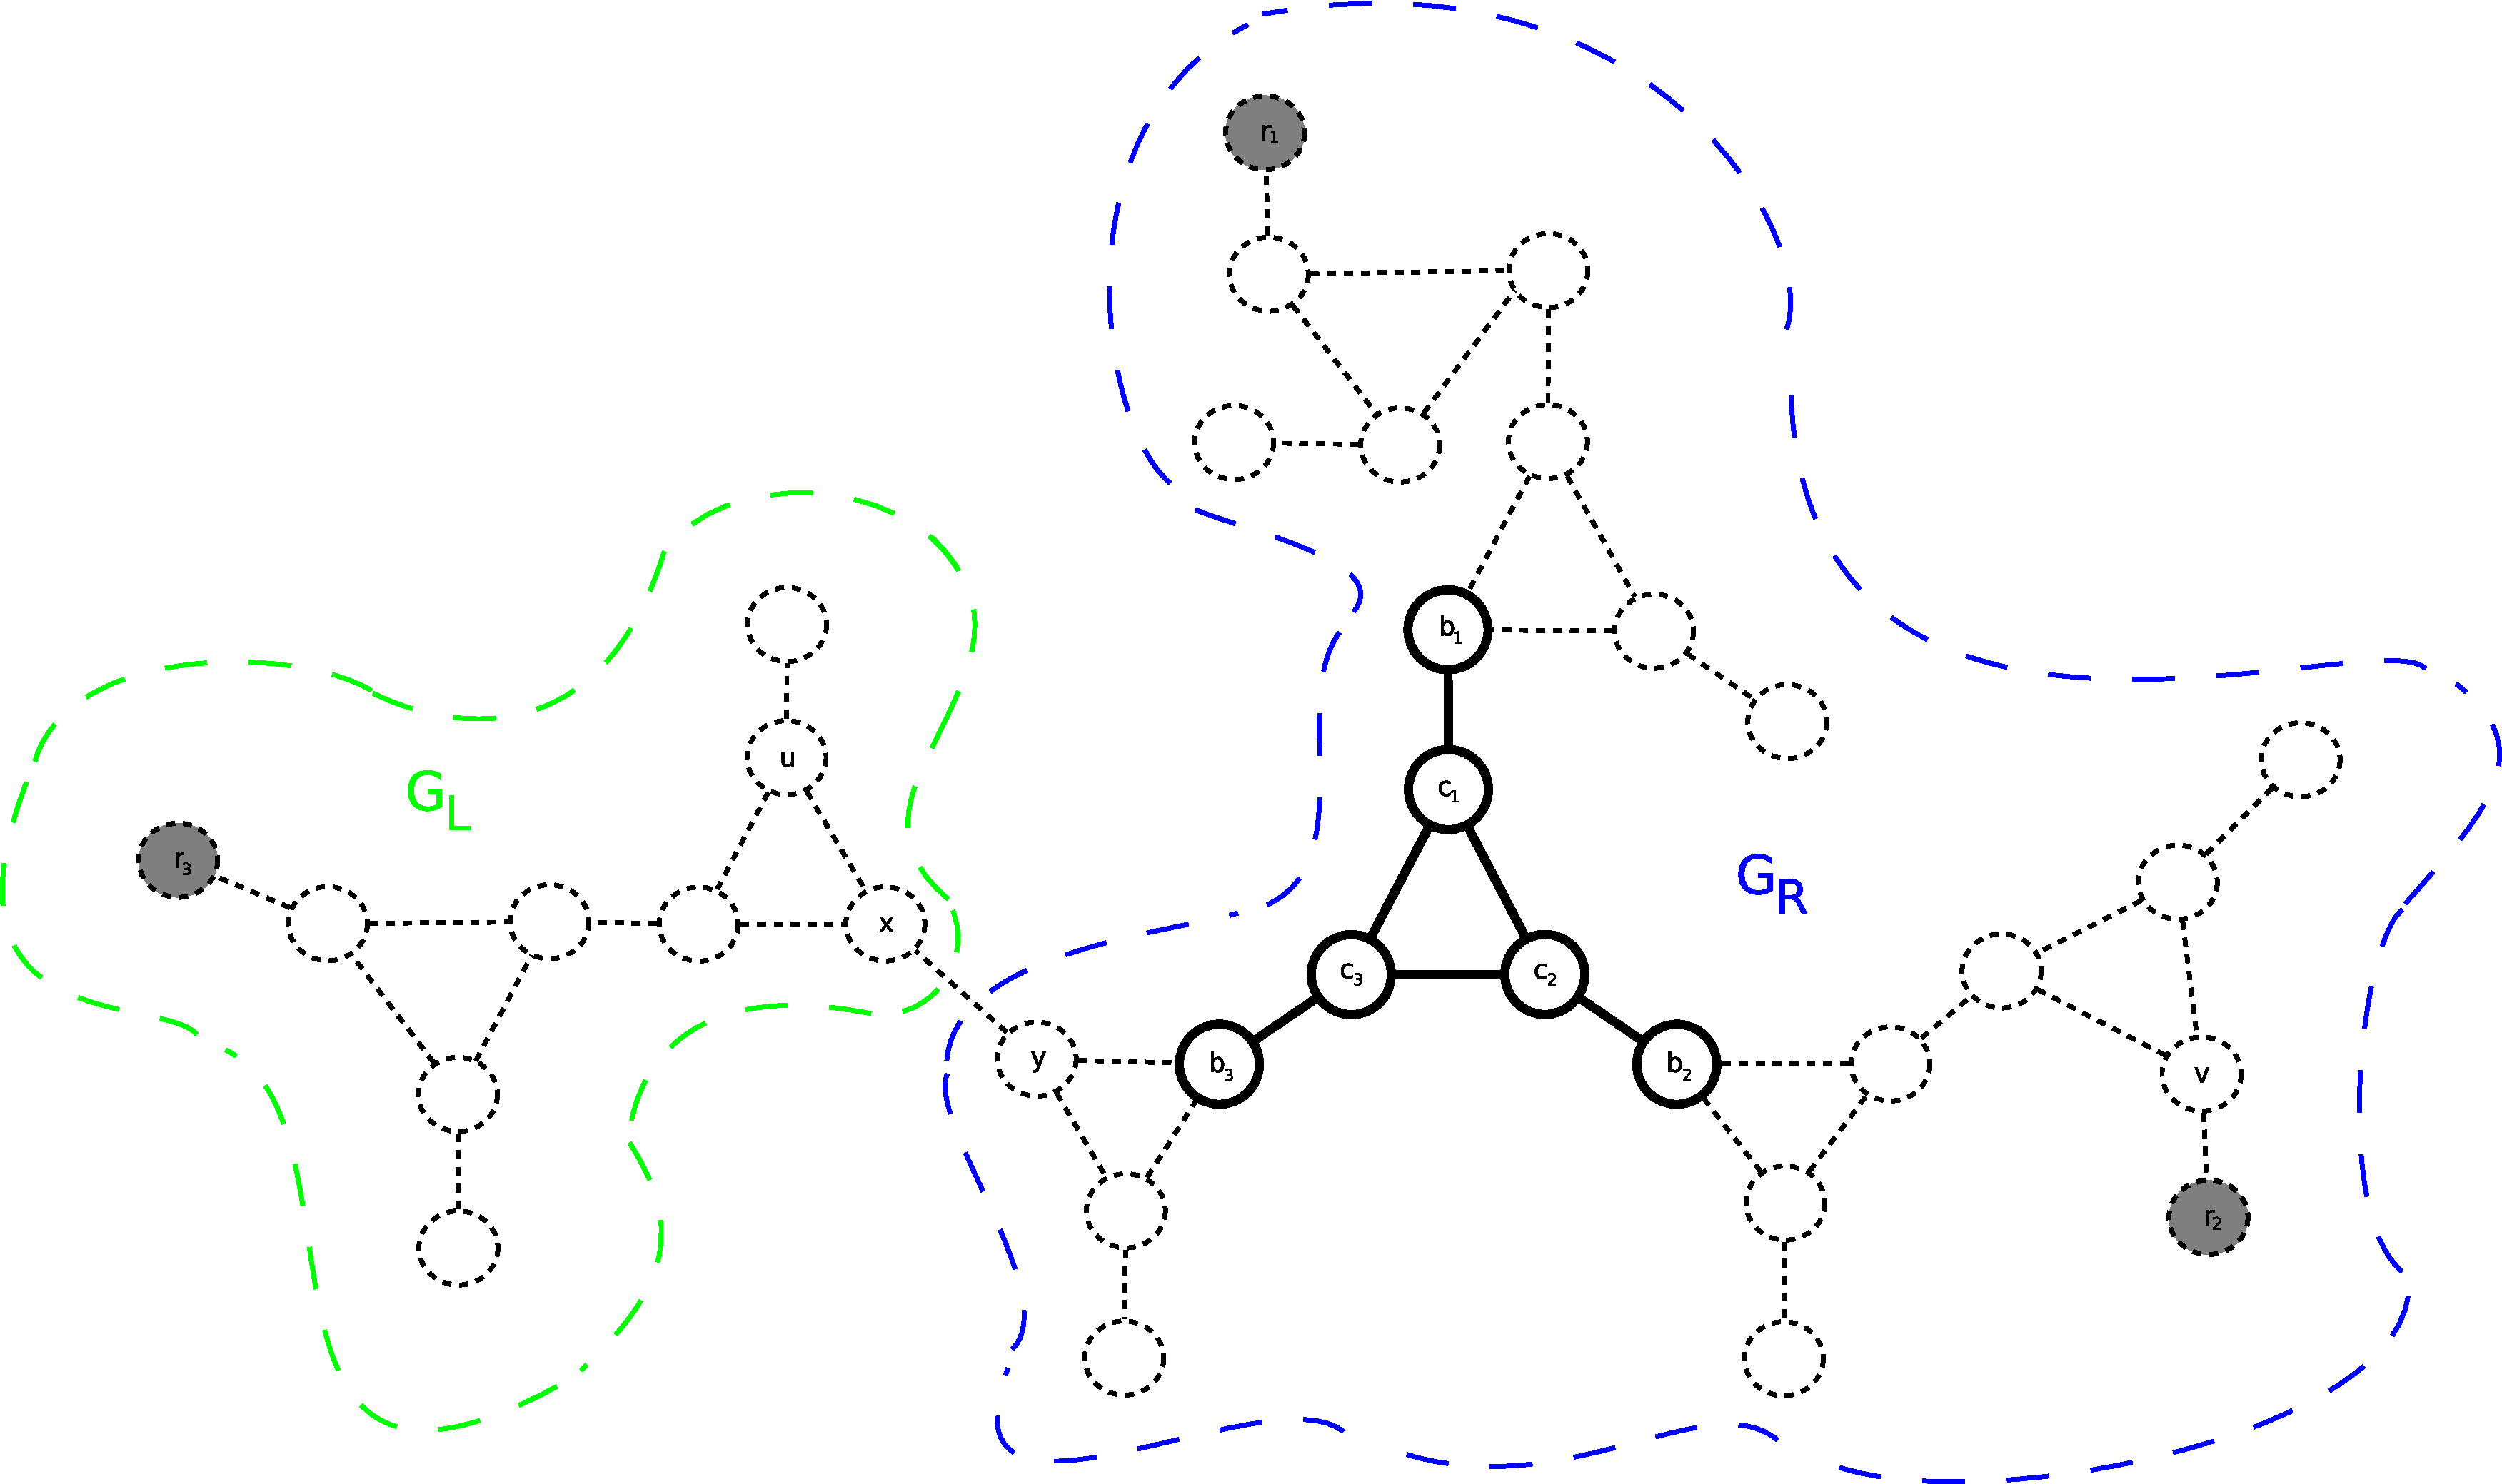
\includegraphics[width=390pt]{bilder/bew2.pdf}
   \caption{Ein Graph mit einem ausgesuchten $C_{3,j}$ und festen $r_1$, $r_2$ und $r_3$}
  	 \end{figure}

\item Fall III. Die Knoten $u$ und $v$ haben die gleiche Distanz vom Knoten $r_1$ aus der metrischen Basis und die Knoten $u$ und $v$ liegen in unterschiedlichen $C_{3,j}$.\\
Der Knoten $u$ hat entweder den Grad eins und ist ein Blatt, welches ein Nachbar eines $C_3$ ist, oder den Grad drei und ist Teil eines festen $C_{3}$. Da der Graph zusammenhängend ist, gibt es in beiden Fällen eine Kante $\{x,y\}$ in dem gleichen $C_{3,j}$ mit der Eigenschaft $x$ Teil von diesem $C_{3}$, $y$ nicht und $dist(v,y) < dist(v,x)$. Durch die zweite Anforderung kann $y$ kein Blatt sein. Nach Lemma \ref{bkb} sind $x$ und $y$ zwei Trennungsknoten, und die beiden nicht zusammenhängenden Graphen, welche durch das Entfernen des jeweiligen Knoten entstehen, haben nach Lemma \ref{bkb2} mindestens ein Element aus der metrischen Basis.\\
Der Teilgraph $G_L$ links von der Kante $\{x,y\}$ beinhaltet den Knoten $u$ und mindestens einen Knoten aus der metrischen Basis $r_3$, der Teilgraph $G_R$ an der anderen Seite der Kante $\{x,y\}$ beinhaltet den Knoten $v$ und mindestens einen Knoten aus der metrischen Basis $r_2$. Nach Satz \ref{first_theorem} sind die Knoten $u$ und $v$ getrennt.
\end{itemize}
\end{proof}
\clearpage
\begin{lem}
\textcolor{white}{x}
\begin{enumerate}
\item Fall: Der Baum besteht nur aus Knoten mit $deg(v) \leq 2$. Damit ist dieser Baum ein Weg und seine metrische Dimension ist eins.\\
\item Fall: Der Baum beinhalten genau einen Knoten mit $deg(v)=3$. Seine metrische Dimension ist zwei.
\end{enumerate}
\end{lem}

%%%%%%%%%%%%%%%%%%%%%%%%%%%%%%%%%%%%%%%%%%%%%%%%%%%%%%%%%%%%%%%%%%%%%%%%%%%%%%%%%%%%%%%%%%%%%%%%%%%%%%%%%%%%%%%%
\subsubsection{Verallgemeinerungen}
Unterschiedliche Möglichkeiten sind für die Verallgemeinerung von $C_3$-Bäumen möglich. Einerseits ist es möglich die Kreisordnung zu erhöhen. Eine andere Möglichkeit ist es jeden Knoten durch einen Kreis, welcher aus sovielen Knoten besteht wie der Grad des ersetzten Knotens, zu ersetzen und jeden Knoten eindeutig einem Nachbarn zuzuordnen.
\begin{comment}
\begin{defi}
For a given tree $T=(V,E)$ with $deg(v_i)\leq 3$ for $v_i \in V$, the $C_j$ Tree is build in the following way: 
   Let $$V'=\{v_k|v_k \in V \wedge deg(v_k)=3\}\subseteq V$$ be a subset of the vertices of the graph $B$. Replace each element $v_j \in V'$ by a $C_k$ with $k \geq 3$ (call this subgraphs \emph{$C_{k,3,j}$}), so that at most one vertex of $C_{k,3,j}$ is connected to exactly one neightbour of $v_j$. The three neightbours of $C_{k,3,j}$ are called the \emph{$C_{k,3,j}$-$children$}. If two of the $C_{k,3,j}$-$children$ are leafs, so the subgraph including the $C_{k,3,j}$ his neighbours is called a \emph{$C_{k,3,j}$-$leaf$}.
\end{defi}
\begin{defi}
For a given tree $T=(V,E)$ with $deg(v_i)\leq n$ for $v_i \in V$, the $C_j$ Tree is build in the following way: 
   Let $$V'=\{v_k|v_k \in V \wedge deg(v_k)=n\}\subseteq V$$ be a subset of the vertices of the graph $B$. Replace each element $v_j \in V'$ by a $C_n$ (call this subgraphs \emph{$C_{n,j}$}), so that exactly one vertex of $C_{n,j}$ is connected to exactly one neightbour of $v_j$. The $n$ neightbours of $C_{n,j}$ are called the \emph{$C_{n,j}$-$children$}. If two of the $C_{n,j}$-$children$ are leafs, so the subgraph including the $C_{n,j}$ his neighbours is called a \emph{$C_{n,j}$-$leaf$}.
\end{defi}

\begin{defi}
For a given tree $T=(V,E)$ with $deg(v_i)\leq n$ for $v_i \in V$, the $C_j$ Tree is build in the following way: 
   Let $$V'=\{v_k|v_k \in V \wedge deg(v_k)=n\}\subseteq V$$ be a subset of the vertices of the graph $B$. Replace each element $v_j \in V'$ by a $C_k$ with $k \geq n$ (call this subgraphs \emph{$C_{k,n,j}$}), so that at most one vertex of $C_{k,n,j}$ is connected to exactly one neightbour of $v_j$. The t$n$ neightbours of $C_{k,n,j}$ are called the \emph{$C_{k,n,j}$-$children$}. If two of the $C_{k,n,j}$-$children$ are leafs, so the subgraph including the $C_{k,n,j}$ his neighbours is called a \emph{$C_{k,n,j}$-$leaf$}.
\end{defi}
\end{comment}
\begin{defi}
Sei ein Baum $T=(V,E)$ mit $deg(v_i)\leq j$ für $v_i \in V$ gegeben. Der $C_j$-$Baum$ resultiert daraus folgend: 
Für alle $3 \leq i \leq j$ und $i \in \mathbb{N}$ sei $$V'=\{v_k|v_k \in V \wedge deg(v_k)=i\}\subseteq V$$ eine Teilmenge der Knoten aus dem Graphen $T$. Ersetze jedes Knoten $v_n \in V'$ durch einen $C_k$ mit $k \geq i$ (bezeichnet wird dieser Teilgraph als \emph{$C_{k,i,n}$}), so dass höchstens ein Knoten von $C_{k,i,n}$ mit genau einem Nachbarn von $v_n$ verbunden ist. Die $i$ Nachbarn von $C_{k,i,n}$ werden als \emph{$C_{k,i}$-$Kinder$} bezeichnet. Sofern zwei dieser $C_{k,i}$-$Kinder$ Blätter sind wird der Teilgraph, welcher den $C_{k,i,n}$ und seine Nachbarn beinhaltet, als \emph{$C_{k,i}$-$Blatt$} bezeichnet.
\end{defi}

\clearpage
\begin{satz}
\end{satz}

%%%%%%%%%%%%%%%%%%%%%%%%%%%%%%%%%%%%%%%%%%%%%%%%%%%%%%%%%%%%%%%%%%%%%%%%%%%%%%%%%%%%%%%%%%%%%%%%%%%%%%%%%%%%%%%%
\subsubsection{Metrische Dimension bei Bäumen und $C_j$-Baümen}
\subsection{Erweiterungen der Radgraphen $W_{1,i,n}$ und $W_{1,n,i}$}
Zwei ähnliche Graphklassen scheinen die Sterne $S_{1,n}$ und die Räder $W_{1,n}$ am Anfang zu sein. Doch ihre Ergebnisse bezüglich der metrischen Dimension sind kernunterschiedlich. Zunächst einmal ist die Eigenschaft nürzlich, dass jeder Sterngraph $S_{1,n}$ ein Teilgraph von dem Radgraphen $W_{1,n}$ ist mit der Eigenschaft, dass die metrische Dimension vom Stern um einiges größer ist, als von dem Rad. (Vergleiche dazu Lemma \ref{sternrad})\\
Interessant ist aber auch die Eignschaft, dass die Erweiterungen vom Stern, die gleiche Dimension haben wie der Stern selbst. Erweitert man beliebig den Graphen beliebig, so bleibt die metrische Dimension gleich. Der Beweis dafür folgt unmittelbar aus dem Satz \ref{trennungsknoten}.\\
Ganz anders ist die Situation bei den Radraphen. Dieses Kapitel widmet sich der Berechnung der metrischen Dimension von erweiterten Radgraphen. Man betrachtet dabei sowohl Erweiterung auf dem äußeren Kreis, wie auch die Erweiterungen zum inneren Knoten.\\

%%%%%%%%%%%%%%%%%%%%%%%%%%%%%%%%%%%%%%%%%%%%%%%%%%%%%%%%%%%%%%%%%%%%%%%%%%%%%%%%%%%%%%%%%%%%%%%%%%%%%%%%%%%%%%%%
%%%%%%%%%%%%%%%%%%%%%%%%%%%%%%%%%%%%%%%%%%%%%%%%%%%%%%%%%%%%%%%%%%%%%%%%%%%%%%%%%%%%%%%%%%%%%%%%%%%%%%%%%%%%%%%%
%%%%%%%%%%%%%%%%%%%%%%%%%%%%%%%%%%%%%%%%%%%%%%%%%%%%%%%%%%%%%%%%%%%%%%%%%%%%%%%%%%%%%%%%%%%%%%%%%%%%%%%%%%%%%%%%
\section{Metrische Dimension von außenplanaren Graphen% ist in $\mathbb{P}$
}

%%%%%%%%%%%%%%%%%%%%%%%%%%%%%%%%%%%%%%%%%%%%%%%%%%%%%%%%%%%%%%%%%%%%%%%%%%%%%%%%%%%%%%%%%%%%%%%%%%%%%%%%%%%%%%%%
%%%%%%%%%%%%%%%%%%%%%%%%%%%%%%%%%%%%%%%%%%%%%%%%%%%%%%%%%%%%%%%%%%%%%%%%%%%%%%%%%%%%%%%%%%%%%%%%%%%%%%%%%%%%%%%%
%%%%%%%%%%%%%%%%%%%%%%%%%%%%%%%%%%%%%%%%%%%%%%%%%%%%%%%%%%%%%%%%%%%%%%%%%%%%%%%%%%%%%%%%%%%%%%%%%%%%%%%%%%%%%%%%
\section{Metrische Dimension von Halin Graphen} 
%%%%%%%%%%%%%%%%%%%%%%%%%%%%%%%%%%%%%%%%%%%%%%%%%%%%%%%%%%%%%%%%%%%%%%%%%%%%%%%%%%%%%%%%%%%%%%%%%%%%%%%%%%%%%%%%
%%%%%%%%%%%%%%%%%%%%%%%%%%%%%%%%%%%%%%%%%%%%%%%%%%%%%%%%%%%%%%%%%%%%%%%%%%%%%%%%%%%%%%%%%%%%%%%%%%%%%%%%%%%%%%%%
%%%%%%%%%%%%%%%%%%%%%%%%%%%%%%%%%%%%%%%%%%%%%%%%%%%%%%%%%%%%%%%%%%%%%%%%%%%%%%%%%%%%%%%%%%%%%%%%%%%%%%%%%%%%%%%%
\section{Zusammenfassung}
\begin{comment}
\begin{table}[htb]
\centering
 \renewcommand{\arraystretch}{1.5} 
\begin{tabular}{|l|c|c|c|c|c|}
\hline
$\:$Protocol & \multicolumn{1}{c|}{WSP} & GTSP & SP & SPP &SSP  \\
\hline
$\:$Cut $\&$ Choose & \Checkmark & \Checkmark  &\Checkmark & \Checkmark &  \XSolidBrush\\
\hline
$\:$Last-Diminisher & \Checkmark & (\Checkmark) & \Checkmark& \Checkmark &  \XSolidBrush\\
\hline
$\:$Lone-Chooser & \Checkmark & \Checkmark  &\Checkmark & \Checkmark &  \XSolidBrush\\
\hline
$\:$Lone-Divider & \Checkmark & \XSolidBrush  & \XSolidBrush &\XSolidBrush & \XSolidBrush \\
%\hline
%$\:$Cut your Own Piece & SPP & SP & \XSolidBrush & \Checkmark &SP& GSP \\
\hline
$\:$Divide-$\&$-Conquer & \Checkmark & \Checkmark &\Checkmark &\Checkmark &  \XSolidBrush \\
\hline
\end{tabular}
\caption{Overview: Strategyproofness of proportional cake-cutting protocols}\label{ov}
\end{table}
\end{comment}
%%%%%%%%%%%%%%%%%%%%%%%%%%%%%%%%%%%%%%%%%%%%%%%%%%%%%%%%%%%%%%%%%%%%%%%%%%%%%%%%%%%%%%%%%%%%%%%%%%%%%%%%%%%%%%%%
%%%%%%%%%%%%%%%%%%%%%%%%%%%%%%%%%%%%%%%%%%%%%%%%%%%%%%%%%%%%%%%%%%%%%%%%%%%%%%%%%%%%%%%%%%%%%%%%%%%%%%%%%%%%%%%%
%%%%%%%%%%%%%%%%%%%%%%%%%%%%%%%%%%%%%%%%%%%%%%%%%%%%%%%%%%%%%%%%%%%%%%%%%%%%%%%%%%%%%%%%%%%%%%%%%%%%%%%%%%%%%%%%
\subsection{Ähnliche Arbeiten}
\begin{comment}
\end{comment}
%%%%%%%%%%%%%%%%%%%%%%%%%%%%%%%%%%%%%%%%%%%%%%%%%%%%%%%%%%%%%%%%%%%%%%%%%%%%%%%%%%%%%%%%%%%%%%%%%%%%%%%%%%%%%%%%
%%%%%%%%%%%%%%%%%%%%%%%%%%%%%%%%%%%%%%%%%%%%%%%%%%%%%%%%%%%%%%%%%%%%%%%%%%%%%%%%%%%%%%%%%%%%%%%%%%%%%%%%%%%%%%%%
%%%%%%%%%%%%%%%%%%%%%%%%%%%%%%%%%%%%%%%%%%%%%%%%%%%%%%%%%%%%%%%%%%%%%%%%%%%%%%%%%%%%%%%%%%%%%%%%%%%%%%%%%%%%%%%%
\section{Offene Fragen und zukünftige Forschung}
\cite{res},\cite{n-3},\cite{OnDet},\cite{Bounds},\cite{Discrep},\cite{Cartesian},\cite{upper},\cite{landmarks}, \cite{Erdos}
\pagebreak

%%%%%%%%%%%%%%%%%%%%%%%%%%%%%%%%%%%%%%%%%%%%%%%%%%%%%%%%%%%%%%%%%%%%%%%%%%
%%%%%%%%%%%%%%%%%%%%%%%%%%%%%%% ENDE TEXTTEIL %%%%%%%%%%%%%%%%%%%%%%%%%%%%
%%%%%%%%%%%%%%%%%%%%%%%%%%%%%%%%%%%%%%%%%%%%%%%%%%%%%%%%%%%%%%%%%%%%%%%%%%

\clearpage
\thispagestyle{empty}
%\vspace*{\fill}g
\pagestyle{plain}
\bibliographystyle{plain}
\bibliography{references}
\thispagestyle{empty}
%\vspace*{\fill}g
\pagestyle{plain}
\clearpage

\listoffigures

\listoftables
\thispagestyle{empty}
%\pagebreak
\pagestyle{plain}
%\printindex
\end{document}
